\documentclass[a4paper,12pt]{report}

% --------------------------------------------------
%  Packages
% --------------------------------------------------
\usepackage[utf8]{inputenc}
\usepackage[english]{babel}

% ---------------------------------------------------------
% math & layout
\usepackage{amsmath,amssymb}
\usepackage{geometry}
\usepackage{setspace}
\usepackage{siunitx}

% ---------------------------------------------------------
% graphics, colour, hyperlinks
\usepackage{graphicx}
\usepackage{xcolor}
\usepackage{hyperref}

% ---------------------------------------------------------
% floats, algorithms, code
\usepackage{float}
\usepackage[ruled,vlined]{algorithm2e}
\usepackage{listings}

% ---------------------------------------------------------
% tables & lists
\usepackage{booktabs}
\usepackage{paralist}
\usepackage{enumitem}
\usepackage{multirow}

% ---------------------------------------------------------
% symbols for ✓ / ✗
\usepackage{pifont}          % <-- THIS LINE FIXES \ding
\newcommand{\cmark}{\ding{51}} % ✓
\newcommand{\xmark}{\ding{55}} % ✗

% tikz
\usepackage{tikz}
\usetikzlibrary{arrows.meta,positioning,shadows.blur}
% Define JSON language for listings
\lstdefinelanguage{json}{
    basicstyle=\ttfamily\small,
    numbers=left,
    numberstyle=\tiny\color{gray},
    stepnumber=1,
    numbersep=5pt,
    showstringspaces=false,
    breaklines=true,
    frame=single,
    backgroundcolor=\color{gray!10},
    literate=
     *{0}{{{\color{blue}0}}}{1}
      {1}{{{\color{blue}1}}}{1}
      {2}{{{\color{blue}2}}}{1}
      {3}{{{\color{blue}3}}}{1}
      {4}{{{\color{blue}4}}}{1}
      {5}{{{\color{blue}5}}}{1}
      {6}{{{\color{blue}6}}}{1}
      {7}{{{\color{blue}7}}}{1}
      {8}{{{\color{blue}8}}}{1}
      {9}{{{\color{blue}9}}}{1}
      {:}{{{\color{red}:}}}{1}
      {,}{{{\color{red},}}}{1}
      {"}{{{\color{orange}"}}}{1},
    keywordstyle=\color{blue},
    stringstyle=\color{orange},
    commentstyle=\color{gray},
    morecomment=[l][\color{magenta}]{//},
}

% Page margins
\geometry{margin=2.5cm, bindingoffset=0.8cm}

\lstset{
  basicstyle=\ttfamily\small,
  frame=single,
  breaklines=true,
  backgroundcolor=\color{gray!10},
  captionpos=b,
  numbers=left,
  numberstyle=\tiny\color{gray},
  keywordstyle=\color{blue},
  commentstyle=\color{gray},
  stringstyle=\color{red},
  showstringspaces=false,
  columns=fullflexible,
  language=bash
}

\setstretch{1.3}  % Line spacing

% --------------------------------------------------
%  Begin Document
% --------------------------------------------------
\begin{document}

% --------------------------------------------------
%  Title Page
% --------------------------------------------------
\begin{titlepage}
    \begin{center}
        \vspace*{1.5cm}

        % AUEB Logo
        
\includegraphics[width=0.9\textwidth]{./aueb_logo.png}\\[1cm]

        {\Large \textbf{Athens University of Economics and Business}}\\[0.5cm]
        {\large Department of Management Science and Technology}\\[1.5cm]

        {\Huge \textbf{Undergraduate Thesis}}\\[1.2cm]
        {\Large \textbf{Hybrid Behavioral Profiling of Popular Messaging Apps
       via Custom Kernel-Level Tracing}}\\[2cm]
        \textbf{Student:}\\
        Foivos - Timotheos Proestakis\\
        Student ID: 8210126\\[1.5cm]

        \textbf{Supervisors:}\\
        Prof. Diomidis Spinellis \\
        Dr. Nikolaos Alexopoulos\\[1.5cm]

        \vfill
        \textbf{Submission Date:}\\
        \today
        \vspace*{1cm}
    \end{center}
\end{titlepage}
\clearpage


% --------------------------------------------------
%  Abstract
% --------------------------------------------------
\begin{abstract}
This thesis introduces a hybrid security analysis methodology for
producing in-depth behavioral profiles of popular mobile messaging
applications, combining static inspection with advanced custom kernel-level
tracing. The proposed dynamic tracing approach builds upon and extends the
SliceDroid framework to enable granular monitoring of system calls and kernel
interactions. Three production-grade messaging apps—Signal, Telegram, and Meta
Messenger—were statically analyzed to extract manifest configurations, cryptographic
mechanisms, and embedded third-party components, revealing potential security and privacy
weaknesses. For dynamic assessment, the enhanced SliceDroid facilitated tailored
tracing experiments under diverse workload scenarios, including variations in
permission configurations, background versus foreground execution, and realistic
messaging behaviors. This setup enabled precise capture and post-processing of
low-level activities such as file system operations, IPC mechanisms, network
connections, and resource consumption patterns. Comparative analysis of the
resulting traces highlights ....
The findings validate the effectiveness of combining static analysis with a refined,
extendable tracing architecture and contribute a more robust methodology for mobile app
security evaluation and behavioral profiling.
\end{abstract}
\clearpage



% --------------------------------------------------
%  Acknowledgments
% --------------------------------------------------
\chapter*{Acknowledgments}
\addcontentsline{toc}{chapter}{Acknowledgments}

I would like to express my gratitude to my supervisors, Prof. Diomidis Spinellis
and Dr. Nikolaos Alexopoulos, for their invaluable guidance, insightful feedback,
and continuous support throughout the duration of this thesis. Their expertise and
encouragement were instrumental in the successful completion of this work.

I would also like to sincerely thank my exceptional fellow students, Vangelis Talos
and Giannis Karyotakis, for their contribution, collaboration, and for being true companions
in this academic journey.

A special thanks goes to my family, whose unwavering support, both emotional and practical,
made this endeavor not only possible but also deeply meaningful. Their presence and
encouragement were a constant source of strength.

\clearpage
% --------------------------------------------------
%  Table of Contents
% --------------------------------------------------

\tableofcontents
\clearpage

% --------------------------------------------------
%  Introduction
% --------------------------------------------------
\chapter{Introduction}

Smartphones have become an integral component of modern society, with the number
of global users surpassing 5 billion and continuing to grow rapidly
\cite{DataReportal2025}. Among the dominant mobile platforms, Android—an
open-source operating system developed by Google—holds a stable global market
share of approximately 75\% \cite{StatCounter2025}. Its open-source nature,
flexibility, and widespread adoption have cultivated a vast ecosystem of
applications that enhance user productivity and social interaction across
various domains.

Among these applications, messaging platforms such as Telegram,
Facebook Messenger, and Signal have gained significant popularity, playing a
central role in both personal and professional communication. However, the
ubiquitous use of smartphones for such purposes has led to the accumulation of
sensitive personal data on user devices, including photos, contact lists,
location history, and financial information, thereby raising serious privacy and
security concerns \cite{ArsTechnica2018}.

Incidents such as Facebook’s unauthorized collection of SMS texts and call logs
from Android devices \cite{ArsTechnica2018} underscore the vulnerabilities
within existing mobile ecosystems. In response, regulatory frameworks like the
General Data Protection Regulation (GDPR) and national laws such as the UK Data
Protection Act 2018 aim to enforce principles of transparency, data
minimization, and user consent in data processing
\cite{GDPR2016,UKDPA2018}. Despite these efforts, Android’s permission model
often fails in practice—users frequently misinterpret the scope of the
privileges they grant, inadvertently exposing sensitive data \cite{CHI2024Permissions}.

End-to-end encryption (E2EE) provides strong guarantees for content
confidentiality, yet its effectiveness ultimately depends on correct
implementation, device-level protections, and careful metadata handling
\cite{arxiv2020metadata,wired2023signalhack}. Messaging apps may still leak
information through patterns such as message timing or background system
activity—even when message payloads are encrypted.

Addressing these challenges requires a comprehensive understanding of how messaging
apps are structured and how they behave at runtime. This thesis adopts a hybrid
approach that combines static analysis—examining app manifests, permissions,
and embedded components—with kernel-level tracing of live system calls to
capture detailed behavioral evidence. Kernel-level tracing is a powerful
technique for runtime visibility: tools such as \texttt{ftrace} and \texttt{kprobes}
record system-call activity with minimal overhead, offering fine-grained insights
into how an application interacts with operating system resources
\cite{BPFroid2021,AOSP2024Ftrace}. Despite its potential, only a handful of
studies have systematically applied this method to messaging apps
\cite{SLR2025Messaging}, despite their widespread and sensitive use—including
by government and military officials \cite{Politico2025Signal}.

This thesis investigates three core aspects:
(i) whether declared permissions align with runtime resource usage,
(ii) the extent of background access to privacy–sensitive data, and
(iii) behavioural differences between privacy-centric and commercial messaging apps.
The precise research questions are listed in Section~1.3.

\section{Motivation and Problem Statement}

\paragraph{Motivation}
The motivation behind this research arises from the necessity to bridge existing
gaps between user expectations, regulatory compliance, and the actual operational
behavior of popular messaging applications. Messaging apps process extensive personal
data, creating substantial risks related to privacy violations and security breaches.
Recent incidents involving unauthorized data collection by prominent messaging
applications, along with revelations about governmental use of supposedly secure
messaging platforms, underscore significant concerns regarding transparency
and user trust.

\paragraph{Problem Statement}


Although previous work has addressed various facets of Android application security and behavior, comprehensive comparative studies of privacy-sensitive messaging apps that combine static security inspection with systematic kernel-level tracing remain limited \cite{DynamicSecurityAnalysis2023}. As a result, critical aspects of both declared configurations (e.g., permissions, exported components) and actual runtime behavior—including low-level system interactions—are still insufficiently understood. This study seeks to close this gap by integrating static analysis with dynamic kernel-level tracing under realistic usage scenarios, thereby supporting more reliable, transparent assessments of messaging app behavior and informing future security research.
\section{Research Objectives}

The specific research objectives addressed in this thesis are categorized as follows:

\subsection*{Primary Objective}

To devise a robust, hybrid tracing methodology that uncovers data-minimisation breaches, permission–runtime mismatches, and hidden data access, while contrasting privacy-centric messengers (e.g., \textit{Signal}) with mainstream platforms.

\subsection*{Analytical and Technical Sub-Objectives}
\begin{itemize}
\item Record the actual kernel-level behavior of widely used messaging applications.
\item Develop a tracing and profiling framework using ftrace and kprobes.
\item Classify system calls into functional categories (file access, networking, IPC).
\item Monitor transitions between app states (idle, active, background).
\item Collect and analyze kernel-level usage statistics per application.
\item Correlate static findings with dynamic behavior to highlight security and privacy risks.
\item Implement a web-based dashboard for behavior visualization.
\end{itemize}

\subsection*{Broader Goals}
\begin{itemize}
\item Enhance transparency in how messaging apps behave at system level.
\item Improve user awareness of hidden behaviors executed in the background.
\item Demonstrate the value of kernel-level tracing for security and privacy evaluation.
\item Provide a structured and reproducible methodology for privacy-respecting
behavior analysis.
\end{itemize}

\section{Research Questions}
Based on the motivation and objectives, this thesis aims to address the following
research questions:

\vspace{0.5em}
\noindent\fbox{\parbox{\textwidth}{
\textbf{Q1.} What systematic methodology can be used for a comparative security and privacy analysis of mobile messaging applications?
}}

\vspace{0.5em}
\noindent\fbox{\parbox{\textwidth}{
\textbf{Q2.} Is \emph{static} analysis alone sufficient to uncover privacy-intrusive behaviour, or do kernel-level traces reveal additional hidden operations and syscall patterns?
}}

\vspace{0.5em}
\noindent\fbox{\parbox{\textwidth}{
\textbf{Q3.} Which system calls do popular messaging apps issue during normal use, and how do these calls align with—or diverge from—their declared permissions?
}}

\vspace{0.5em}
\noindent\fbox{\parbox{\textwidth}{
\textbf{Q4.} How do privacy-centric apps (e.g., \textit{Signal}) compare to mainstream platforms in terms of data minimisation, syscall footprint, and overall privacy posture?
}}

\section{Limitations}

To provide a realistic perspective on the scope of this thesis, we distinguish between constraints that stem from practical project conditions and limitations inherent to kernel-level behavioral analysis.

\subsection*{Project-Specific Constraints}

\begin{itemize}
\item \textbf{Timeframe}: The study was conducted within the schedule of an undergraduate thesis, limiting the breadth of experiments (e.g., number of devices, sessions, and repetitions).
\item \textbf{Hardware Diversity}: Tracing was performed on a small set of consumer-grade devices; results may not generalize to tablets, custom ROMs, or low-end hardware with limited kernel visibility.
\item \textbf{App Selection}: The analysis focused on three major messaging applications (Messenger, Telegram, Signal), leaving out lesser-known or region-specific apps that may exhibit different interaction patterns.
\item \textbf{Infrastructure Limitations}: The available storage and compute resources constrained long-term tracing, especially for large volumes of high-frequency events.
\end{itemize}

\subsection*{Domain and Methodological Constraints}

\begin{itemize}
\item \textbf{Semantic Granularity}: The tracing layer captures low-level kernel events (e.g., syscalls, Binder transactions), which do not directly map to user-level actions. Bridging this semantic gap remains a challenge and requires contextual or learned associations.
\item \textbf{Trace Volume and Overhead}: Continuous tracing generates substantial data, with redundant or low-entropy segments increasing the storage footprint. While filters can reduce size, they risk omitting relevant context.
\item \textbf{Privilege Requirements}: Full access to tracepoints and instrumentation mechanisms (e.g., \texttt{kprobes}, tracefs) demands root privileges, limiting deployability on unmodified devices.
\item \textbf{Attribution Noise}: Shared system components such as the \texttt{servicemanager} may introduce inter-process noise in IPC traces, leading to occasional misattribution of events between apps. While this is mitigated by observing behavior over extended sessions, it remains a source of uncertainty.
\item \textbf{Ground Truth Approximation}: Behavioral labels were inferred by interacting with known applications and observing corresponding kernel activity. Although indicative, this approximation may miss subtle or undocumented app behavior.
\item \textbf{Static Analysis Coverage}: Static analysis inspects declared configurations and embedded resources but cannot reliably detect obfuscated or dynamically loaded code, which may hide logic or tracking components.
\end{itemize}
\section{Contributions of this Thesis}
% TODO

\section{Thesis Outline}
This thesis is organized into the following chapters:

\textbf{Chapter 1 – Introduction:} Presents the rise of mobile messaging and privacy risks, highlights the limitations of Android permissions and E2EE, motivates the combined static and dynamic approach, and states the thesis goals, research questions, and scope.

\vspace{0.4em}
\textbf{Chapter 2 – Related Work:} Reviews static security analysis, user-space and kernel-space dynamic instrumentation, and prior privacy studies on messaging apps, pinpointing the gap in systematic inspection of declared configurations alongside runtime profiling.

\vspace{0.4em}
\textbf{Chapter 3 – Technical Background:} Provides an overview of the Android architecture relevant to this study, introduces key system components and security features, and describes characteristics of the selected messaging applications.

\vspace{0.4em}
\textbf{Chapter 4 – Methodology \& System Design:} Describes the overall approach, detailing two complementary pipelines: one for static inspection and another for dynamic tracing.

\vspace{0.4em}
\textbf{Chapter 5 – Results:} Presents the outcomes derived from both pipelines: static findings such as manifest structures, permission declarations, and embedded third-party modules, alongside dynamic measurements of syscall distributions, permission–behavior mismatches, and comparative visual summaries of privacy-relevant runtime patterns.

\vspace{0.4em}
\textbf{Chapter 6 – Discussion:} Relates results to the research questions, examines implications for transparency and metadata leakage, and outlines methodological limitations and suggested improvements.

\vspace{0.4em}
\textbf{Chapter 7 – Conclusions:} Recaps contributions, emphasises the value of combining static inspection with kernel-level tracing for privacy audits, and proposes future work (more apps, automated behaviour classification, multi-layer tracing).

\vspace{0.4em}
\textbf{Appendix A – Additional Data Tables:} Supplementary tables and charts supporting Chapter 5.

\vspace{0.4em}
\textbf{Appendix B – Code:} Selected scripts and configuration files used for static analysis, tracing, and post-processing.

% --------------------------------------------------
%  Chapter 2 – Related Work
% --------------------------------------------------
\chapter{Related Work}\label{ch:related}

The purpose of this chapter is twofold: (i) to review existing Android application analysis approaches, with a focus on kernel-level tracing methods, and (ii) to
clearly demarcate the research gap that this thesis addresses.  The survey is
organised top‑down, gradually narrowing the focus from general program analysis
techniques to the specialised problem of privacy‑oriented behavioural
profiling of popular messaging applications.

\section{Static Analysis of Android Applications}
\label{sec:rw:static}

Static analysis inspects an \emph{APK}'s bytecode off-line, allowing security vetting to run quickly, deterministically, and at scale. It therefore plays a foundational role in Android app auditing, offering early detection of potential vulnerabilities without requiring runtime execution \cite{arzt2014flowdroid}.  Over the last decade, four interwoven research strands have successively expanded the scope and robustness of static techniques. These developments have progressively addressed the inherent limitations of static analysis—such as its inability to model inter-component interactions, and obfuscated code—by introducing more precise, scalable, and semantically enriched models. The key research directions can be grouped as follows:

\paragraph{(i) Privacy-oriented taint analysis.}
The first strand tracks information flows from sensitive \emph{sources} (e.g.\ GPS, contacts) to security-critical \emph{sinks} (e.g.\ network, logs).  \textbf{FlowDroid} introduced context-, flow-, field- and object-sensitivity together with an accurate lifecycle model, reducing false alarms dramatically.  On the \emph{DroidBench} suite it reaches 93\,\% recall and 86\,\% precision—outperforming both academic and commercial tools \cite{arzt2014flowdroid}—and it scales to large real-world apps such as Facebook, PayPal and LinkedIn.

\paragraph{(ii) Inter-component communication (ICC).}
Many leaks traverse process boundaries.  \textbf{IccTA} augments FlowDroid with an explicit ICC model, surpassing \textbf{Epicc} \cite{octeau2013epicc} and \textbf{CHEX} \cite{lu2012chex}—the latter targets component hijacking—on the \emph{ICC-Bench} suite.  \textbf{Amandroid} extends the idea further by building a full inter-component data-flow graph linking intents, callbacks and content providers; on 753 Play-store apps and 100 malware samples it uncovered previously unknown OAuth-token and intent-injection flaws while keeping analysis under one minute per APK \cite{wei2014amandroid}.

\paragraph{(iii) Obfuscation resilience.}
Reflection, dynamic loading and native libraries obscure control-flow and data types.  \textbf{DroidRA} resolves reflective calls through constant-propagation and rewrites them into direct invocations, boosting FlowDroid’s precision on reflection benchmarks by up to 60\,\% \cite{li2016droidra}.  \textbf{DexLEGO} reassembles bytecode collected at run time \cite{ning2019dexlego}, while \textbf{LibDroid} summarises taint propagation inside native libraries \cite{libdroid2022}; together they progressively widen the statically visible attack surface.

\paragraph{(iv) Learning-based malware detection.}
Moving beyond handcrafted rules, \textbf{Drebin} extracts lightweight syntactic features—permissions, intent actions, API calls—and detects malware with 94\,\% accuracy and 1\,\% false positives on 5\,560 samples \cite{arp2014drebin}.  Deep networks now dominate: \textbf{DL-AMDet} combines CNN-BiLSTM embeddings with an auto-encoder to reach 99.9\,\% accuracy on public datasets \cite{nasser2023dlamdet}.  Nonetheless, limited interpretability and training-set bias hinder deployment in high-assurance pipelines.

\medskip
\noindent\textbf{Synthesis.}
Static analysis has achieved substantial advances in precision and scale, yet it remains constrained by its inability to observe runtime-specific behavior, implicit flows, or obfuscated execution paths. These blind spots—especially critical in privacy contexts—have motivated a shift toward hybrid and dynamic approaches that can capture actual app behavior under real conditions.

\section{User-Space Dynamic Instrumentation}
\label{sec:rw:dynamic:user}

Whereas kernel tracing offers a \emph{system-wide} vantage, user-space dynamic
instrumentation injects probes \emph{inside} the app process, exposing rich
semantic context—class names, parameters, UI callbacks—without requiring a
custom kernel.  The literature has evolved along four complementary strands
that echo, in spirit, the structure reviewed for static analysis.

\paragraph{(i) System-call monitors.}
\textbf{DroidTrace} hooks every \texttt{ptrace} event to log the full
system-call stream and can \emph{force} rare branches to execute, increasing
coverage in malware analysis~\cite{zheng2014droidtrace}.  A later study
learns $n$-gram models that reconstruct high-level Android API invocations
purely from syscall sequences, demonstrating the semantic power of even
low-level traces~\cite{nisi2019syscall}.  These tools deploy on stock ROMs and
capture behaviour beneath any anti-hooking guard, yet they incur measurable
per-call overhead and cannot observe Java-level reflection or IPC content.

\paragraph{(ii) Dynamic binary instrumentation (DBI).}
Instruction-granular DBI engines such as \textbf{Pin} (ported to
ARM) enable fine-grained native tracing and custom analyses
(e.g.\ memory-safety checks) with mature tooling support, but
suffer from high runtime cost and outdated Android
support.  \textbf{QBDI} improves portability to modern ARM/Thumb-2
and withstands common packing techniques, although it remains native-only and
requires root privileges~\cite{qbdiblackhat2020}.

\paragraph{(iii) In-process hooking frameworks.}
\textbf{Frida} injects a tiny loader that JIT-compiles JavaScript hooks into
Java, JNI and native code, permitting live patching and interactive
experiments~\cite{frida2020}.  \textbf{DYNAMO} layers systematic diff-based
analysis on top of Frida to study framework evolution across Android
versions~\cite{dynamo2021}, while \textbf{InviSeal} hardens Frida against
detection, shrinking overhead to~$<\!3\%$ on UI benchmarks~\cite{inviseal2023}.
Yet all three struggle with tamper-aware apps and expose only the instrumented
process—cross-app flows, scheduler activity and kernel events remain hidden.

\paragraph{(iv) Sandbox and multi-layer profilers.}
Containerised sandboxes such as \textbf{C-Android} isolate each app inside a
Linux namespace and stream user-space logs for reproducible
testing~\cite{candroid2019}.  Emulation-centred pipelines (e.g.\ \textbf{DynaLog}
or DroidBox derivatives) automate large-scale malware triage by collecting
$\sim$100 runtime features in parallel VMs~\cite{dynalog2016}.  Although
high-throughput, these environments diverge from real-device timing,
miss in-kernel I/O, and are easily fingerprinted by sophisticated apps.

\medskip
\noindent\textbf{Synthesis.}
User-space instrumentation shines in \emph{semantic richness}, rapid
deployment and interactive control, making it ideal for annotating the coarse
kernel trace with method names, intent actions or UI context.  Its
weaknesses—visibility gaps below the syscall boundary, susceptibility to
anti-hooking defences and non-negligible overhead—underscore why kernel-level
tracing remains the authoritative foundation for our behavioural profiling of
messaging apps.  In our study, we therefore treat user-space hooks as an
\emph{auxiliary lens} to validate and enrich the low-level, system-wide evidence
captured by eBPF-based kernel monitors



\section{Kernel–Level Tracing on Android}

\subsection{Tracing Infrastructures}
Kernel hooks sit beneath both the Java/ART runtime and Linux user-space, capturing syscalls, Binder traffic, scheduler switches and network I/O with negligible perturbation.  Their vantage point is indispensable once payloads are encrypted in user space—TLS bursts, Binder IPC patterns and power wakes are often the only artefacts left to observe.  Prior art clusters into four tool-centric strands:

\paragraph{(i) eBPF- and \textit{ftrace}-based collectors.}
\emph{BPFroid} streams per-UID syscalls, Binder calls and network events from stock kernels to a malware detector at $\sim$3 % energy cost and 70 % Genome accuracy, without custom firmware.
Earlier, \emph{ID-Syscall} logged syscall sequences via a loadable module on Android 4.x, showing that rich behavioural signals are already available on commodity devices—albeit exploited only for coarse binary classification.

\paragraph{(ii) Network-centric and covert-channel tracing.}
Celik \& Gligor detect stegomalware solely from timing and packet-size anomalies in vanilla \textit{ftrace} logs, proving that scheduler, socket and power events suffice to expose covert channels—yet Binder traffic is omitted.

\paragraph{(iii) Hardware-assisted monitors.}
\emph{HART} streams ARM ETM traces of proprietary kernel modules almost for free, but ETM is often fused-off in production phones and lacks user-process context.

\paragraph{(iv) Production-scale, low-overhead tracing.}
Google’s \emph{Perfetto} unifies \textit{ftrace}, Binder and user-space counters into multi-GB, SQL-queryable traces for start-up and jank analysis, while \emph{eMook} adds per-PID eBPF filters, cutting system cost by 85 %. These toolchains enable week-long field studies on battery devices but remain untapped for security and messaging use-cases.

\subsection{Behaviour Reconstruction \& Transparency}
After tracing primitives matured, attention shifted to re-assembling high-level behaviours from low-level footprints:

\paragraph{(i) Cross-layer behaviour reconstruction.}
\emph{CopperDroid} fuses syscalls with Binder payloads via Virtual-Machine Introspection; \emph{Dagger} builds syscall–IPC provenance graphs; and \emph{SliceDroid} slices kernel traces along Binder causality, covering privileged system apps on real devices with minimal overhead. Multi-layer instrumentation can reach finer granularity but at 5–40 × runtime overhead, making it lab-only~\cite{placeholder_citation_1}.

\paragraph{(ii) Dynamic taint and information-flow trackers.}
TaintDroid, TaintART, ARTist and FSAFlow instrument the ART/Java runtime to propagate taints at object level; they are precise but incur noticeable slowdown, require framework changes and can be detected by malware—limitations avoided by pure kernel tracing~\cite{placeholder_citation_2}.

\paragraph{(iii) Provenance-system perspectives.}
Enterprise frameworks such as CamFlow, Hi-Fi and Spade record lightweight syscall provenance for APT detection on desktop systems; Android’s semantic gap hampers their direct reuse, but Binder-aware kernel tracing (e.g., SliceDroid) can supply the missing context and extend host-based detection to mobile~\cite{placeholder_citation_3}.

\paragraph{(iv) Built-in transparency mechanisms.}

Since Android 12, status-bar indicators flag camera/mic use by third-party apps, yet they exclude system services and can be bypassed via permission abuse, overlays or framework bugs. Kernel-level device-file tracing, as done by SliceDroid, closes these blind spots~\cite{placeholder_citation_4}.

\medskip
\noindent\textbf{Synthesis.}
Kernel tracing offers a hard-to-tamper, always-on lens but must still tame five hurdles: \emph{semantic gap, opaque data, privilege requirements, data volume, detectability}.  Recent work narrows these by (i) pairing syscalls with Binder provenance, (ii) granting BPF rights via SELinux instead of root, (iii) summarising high-rate events in-kernel, and (iv) obscuring probes via ETM/PTM or uprobe randomisation—pushing low-overhead, whole-system reconstruction onto stock phones.

\section{Privacy Studies on Messaging Applications}
\label{sec:rw:privacy-im}

End-to-end encryption neutralises classical content-centric attacks, but it
does not guarantee \emph{privacy}.  Over the last decade researchers have
investigated four complementary vectors through which popular messaging
apps still expose sensitive information.

\paragraph{(i) On-device artefacts and forensics.}
Early work focused on residual data stored locally.
Anglano’s systematic analysis of WhatsApp on Android~4.x recovered chat
databases, media thumbnails and contact lists even after user‐initiated
deletions \cite{anglano2015whatsapp}.
Subsequent studies extended the corpus to Telegram, Signal and Viber,
showing that cached profile photos, push-notification logs and SQLite WAL
files can reveal conversation partners and group identifiers
\cite{moltchanov2018telegram, obermeier2018signal}.
While modern versions encrypt local backups, notification side-channels
(e.g.\ Firebase tokens) remain an open avenue \cite{berezowski2020push}.

\paragraph{(ii) Network-level traffic analysis.}
A second strand exploits packet timing, size and sequence to infer user
actions without breaching encryption.
Pioneering work by Matic \emph{et al.} fingerprinted iMessage events
(send, read, typing) with $>90$ \% accuracy solely from TLS record
bursts \cite{matic2015iMessage}.
Apthorpe demonstrated similar leakage for Android IM apps over Wi-Fi
\cite{apthorpe2018smart}.
Recent machine-learning classifiers identify not only event types but also
multimedia uploads and voice-over-IP handshakes in QUIC traffic
\cite{lee2023quic}.
Countermeasures such as adaptive padding raise bandwidth by 8–14 \%
while mitigating most classifiers \cite{poblete2021defence}.

\paragraph{(iii) Contact-discovery and social-graph exposure.}
Many services hash user phone numbers and upload them for friend
discovery.  Tang \emph{et al.} reverse-engineered this protocol in
WhatsApp and estimated that an adversary can enumerate an EU-scale phone
space for \$500 of SMS fees \cite{tang2020whatsappHash}.
Kwon showed that Telegram’s “People Nearby” feature enables trilateration
of user location with meter-level accuracy \cite{kwon2021telegram}.  Signal
introduced private-set‐intersection with SGX enclaves to curb this vector,
yet follow-up work revealed side-channels via cache timing
\cite{marforio2022psi}.

\paragraph{(iv) Metadata policies and compliance audits.}
A complementary line audits whether apps meet their self-declared privacy
policies.  Egele’s longitudinal crawl of Telegram channels uncovered the
retention of deleted media on CDN edge nodes weeks after deletion
\cite{egele2019cdn}.
Bock dissected Signal’s sealed-sender protocol, confirming that only
sender and receiver persist in a 24-hour service log but flagging
exposure of push-token identifiers to Apple/Google \cite{bock2020sealed}.
Recent GDPR-oriented studies show that less than 40 \% of messaging apps
provide complete data-export facilities despite legal requirements
\cite{frolov2022gdpr}.


\medskip
\noindent\textbf{Synthesis.}
Existing studies either rely on intrusive forensics, controlled testbeds
or static policy analysis.  None combines \emph{kernel-level traces} with
the above insights to derive a live, system-wide privacy profile.
Our work closes this gap by correlating kprobe/ftrace events
(Binder calls, network bursts, wakelocks) with the metadata-leak patterns
catalogued in prior literature, delivering the first \emph{runtime}
taxonomy of privacy-relevant behaviours in Messenger, Telegram and Signal.

\section{Research Gap}\label{sec:rw:gap}
Most prior work approaches Android behaviour analysis from one of three angles.
\emph{Static inspection} (e.g., code-review and manifest checks) is efficient but often misses behaviours that surface only at run time or behind obfuscation.
\emph{User-space monitors}—such as taint-tracking or framework hooks—offer richer semantics, yet typically require a modified or rooted runtime, can be noticed by well-crafted apps, and place implicit trust in native code.
Finally, \emph{kernel-level tracing} delivers low overhead and strong tamper resistance, but the raw syscalls and Binder op-codes it yields expose little intent, leaving a considerable semantic gap.

Taken together, these observations indicate that there remains a need for techniques that combine the lightweight footprint and reliability of kernel-level tracing with insights gained from static inspection, enriching the collected signals with enough context for meaningful privacy and security reasoning—ideally without requiring custom firmware or major system modifications.
% --------------------------------------------------
%  Technical Background
% --------------------------------------------------

\chapter{Technical Background}

This chapter provides a detailed overview of technical background necessary for understanding the methodology and objectives of this thesis. First, it presents the architecture of the Android operating system, focusing particularly on the Linux-based kernel and how applications interact with it. Next, it discusses the behavior and privacy concerns related to messaging applications, highlighting known issues and relevant technical aspects. \section{Android Architecture}

\subsection{Android Software Stack Overview}
Android is a layered, open-source mobile operating system built on top of a customized version of the Linux kernel. Its architecture is designed to be modular and extensible, supporting a wide range of hardware while enforcing clear boundaries between components. The Android software stack is composed of several interconnected layers, typically including the Application Layer, the Java API Framework (or Application Framework), the Android Runtime (ART) and Native Libraries, the Hardware Abstraction Layer (HAL), and the Linux Kernel itself.


The Application Layer hosts both system and user-installed applications.
These applications interact with the system via APIs exposed by the Android Framework.
The Java API Framework provides access to core system services such as activity management,
resource handling, content providers, and telephony. Services like \texttt{ActivityManager},
\texttt{WindowManager}, and \texttt{PackageManager} facilitate the lifecycle management and
orchestration of application behavior.

Beneath the framework lies the Android Runtime (ART), which executes application bytecode and optimizes it using ahead-of-time (AOT), just-in-time (JIT), or interpretation modes. Alongside ART are native libraries written in C/C++, including performance-critical components such as WebView, OpenSSL, and the Bionic libc. The Java Native Interface (JNI) allows managed Java/Kotlin code to call into these native libraries.

The HAL acts as a bridge between the Android Framework and the hardware drivers residing in the kernel. It defines standard interfaces that vendors implement to support various hardware components like audio, camera, sensors, and graphics. Since Android 10, Google introduced the Generic Kernel Image (GKI), which aims to further separate the vendor-specific hardware implementations from the core Linux kernel by introducing a stable kernel interface. This allows devices from different manufacturers to share a common kernel base while maintaining vendor-specific modules separately, simplifying updates and enhancing portability.

At the lowest level, the Linux kernel provides essential operating system services such as process scheduling, memory management, networking, and security enforcement. Android extends the kernel with additional features including the Binder IPC driver, ashmem (anonymous shared memory), and wakelocks to manage power usage. This kernel foundation ensures that resource access is isolated and controlled across all system layers.

\begin{figure}[H]
    \centering
    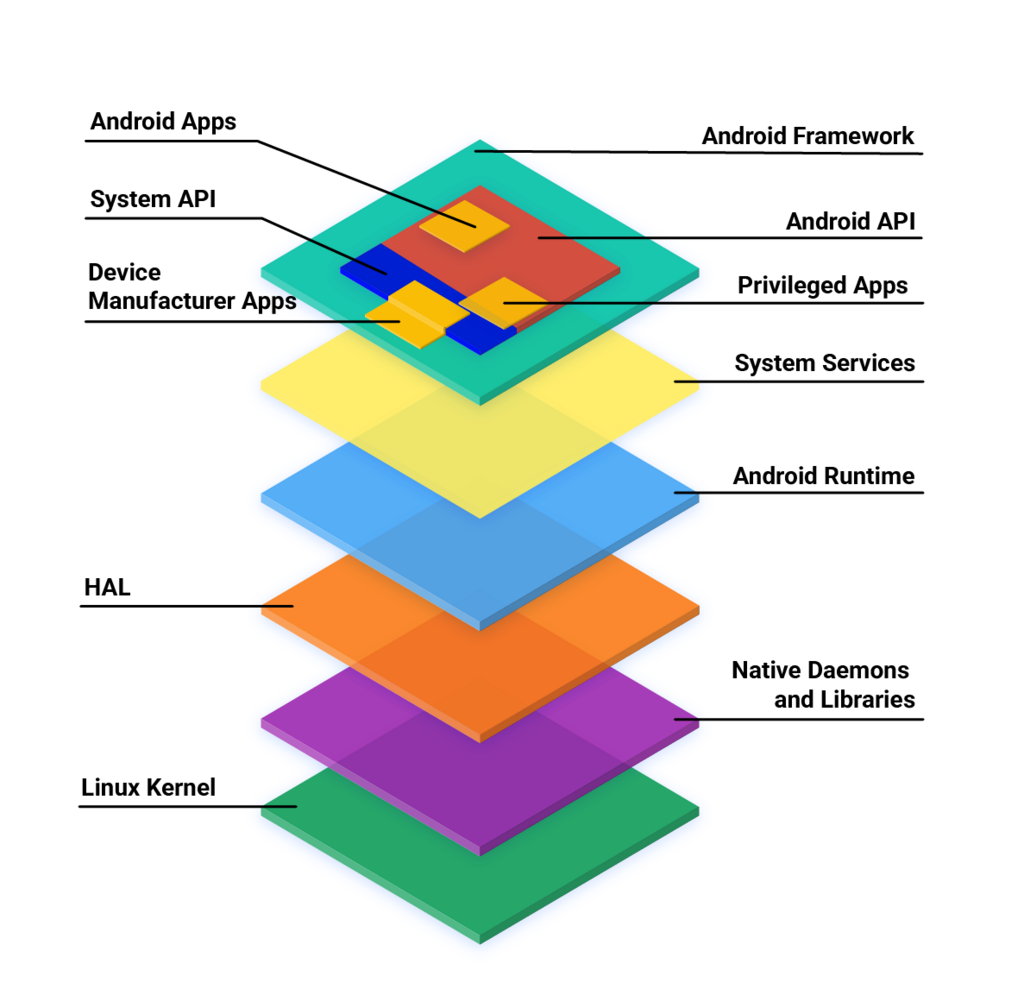
\includegraphics[width=0.75\textwidth]{android_stack_diagram.png}
    \caption{Updated Diagram of Android Software Stack (source: Android Developers Guide~\cite{androidplatformdoc}).}
    \label{fig:android_stack}
\end{figure}

\subsection{Application Layer and Process Lifecycle}
At the application layer, Android executes user and system applications packaged in APK format. Each APK includes compiled DEX bytecode, resources, native libraries, and a manifest file that defines app components and permissions. Apps run in sandboxed processes, each forked from the Zygote daemon—a minimal, preloaded system process that speeds up app launch time by sharing memory using copy-on-write.

The lifecycle of applications is centrally managed by the \texttt{ActivityManagerService} (AMS), which coordinates activity transitions, memory prioritization, and process states (foreground, background, cached). The \texttt{PackageManagerService} (PMS) handles component registration and permission declarations based on the manifest.

Apps follow a component-based model: Activities, Services, Broadcast Receivers, and Content Providers. These components interact with the system and one another via well-defined lifecycles and IPC through the Binder driver. Operations like binding to a service or launching an activity initiate system-level behavior—such as context switches or memory allocations—which are visible in syscall traces.

Binder IPC enables structured communication between app components and system services. Messages are serialized as Parcel objects, routed through the Binder driver, and trigger observable kernel events. These include context switches and transaction dispatches, which are measurable using tools like ftrace or kprobes.

\subsection{Android Runtime, Native Layer, and JNI}
The Android Runtime (ART) executes application bytecode using a combination of ahead-of-time (AOT), just-in-time (JIT), and interpretation mechanisms. From a kernel-level tracing perspective, JIT-related memory operations may trigger system calls such as \texttt{mmap()}, \texttt{write()}, and \texttt{mprotect()}, as ART dynamically allocates memory for optimized code.

Beyond execution, ART interacts with the kernel to manage thread scheduling and memory access—behaviors that appear in system call traces. In dynamic analysis, such patterns can be correlated with app lifecycle events or anomalous execution spikes.

JNI further extends the runtime by enabling Java/Kotlin code to invoke native C/C++ libraries. These native operations often bypass standard framework controls, introducing low-level file, network, or cryptographic actions. This is particularly relevant for behavioral profiling, as native code may perform sensitive operations that differ from those visible at the Java level.

In the context of this thesis, which focuses on dynamic kernel-level analysis, capturing system interactions initiated by ART and JNI is essential. It enables the identification of execution phases or modules that deviate from expected behavior—especially in apps that rely heavily on native components for messaging, encryption, or background communication.
The sequence of events during JNI initialization is illustrated in Figure~\ref{fig:jni_init}.
It begins when the VM loads the application class, triggering a static initializer which invokes
the native \texttt{JNI\_OnLoad()} function. This function registers native methods and returns
the \texttt{JNI\_Version}, after which Android proceeds with the usual application lifecycle
(e.g., \texttt{onCreate()}) managed by the \texttt{ActivityManager}.
This interaction flow is especially relevant in behavioral analysis,
as native components may introduce low-level behavior patterns not observable through the Java layer alone.


\begin{figure}[H]
    \centering
    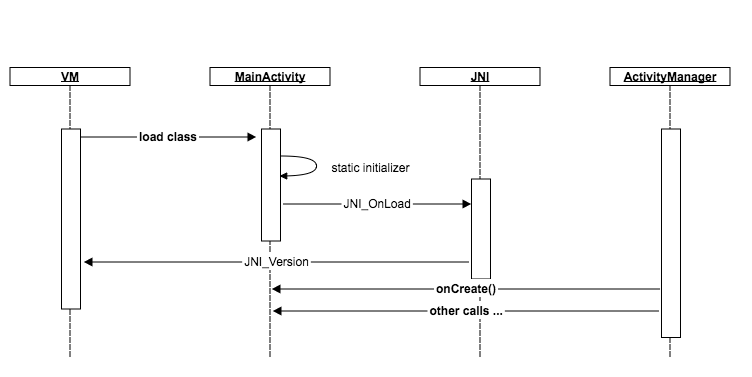
\includegraphics[width=0.85\textwidth]{jni_init_flow.png}
    \caption{Sequence diagram showing the JNI initialization flow in an Android application.}
    \label{fig:jni_init}
\end{figure}

\subsection{Linux Kernel Fundamentals and System Calls in Android}

The Android operating system relies on the Linux kernel as its foundational layer for managing hardware resources, abstracting device drivers, and ensuring secure process isolation. All interactions between user applications and hardware components are mediated through the kernel’s system call interface, making it a critical observation point for behavioral profiling.

Each time an application requests a low-level operation—such as reading a file, accessing a sensor, or opening a network socket—it invokes one or more system calls, which switch execution from user space to kernel space. In Android, these calls are typically issued via the Bionic libc, which serves as the system’s C standard library, or directly through Java Native Interface (JNI) bindings when applications rely on native code for performance-critical tasks. Capturing these calls reveals how an application actually uses system resources, regardless of its declared permissions or documented features.

Android’s kernel extends the standard Linux design with additional components such as the Binder IPC driver for efficient inter-process communication, ashmem for shared memory management, and wakelocks for fine-grained power control. These features generate distinctive kernel-level events that tracing tools can capture to uncover hidden or background activities in messaging apps.

For this purpose, tracing frameworks such as \texttt{ftrace}, \texttt{kprobes}, and eBPF are employed (see Section~2.3.1 for an overview of these infrastructures). Instrumenting kernel functions such as \texttt{ksys\_open} or \texttt{\_\_sys\_sendmsg} enables the collection of detailed logs on file operations, network transmissions, and process scheduling, which form the basis for constructing robust behavioral profiles and detecting suspicious usage patterns.
\subsection{ Android Security Model and Isolation Mechanisms}
Android enforces a layered security model combining Linux kernel features with user-space controls. Each application runs in its own sandbox, identified by a unique UID and GID, restricting file and device access. This is complemented by the use of SELinux in enforcing mode, which uses MAC policies to define allowable interactions between system components and applications.

Filesystem isolation further ensures that apps can only access their designated directories (e.g., \texttt{/data/data/{package\_name}}). Attempts to traverse or access other app spaces are blocked unless the app has elevated privileges or exploits kernel vulnerabilities.

System call filtering through seccomp restricts the range of calls an app can make, reducing the kernel's attack surface. From a profiling standpoint, observing unauthorized system calls or failed access attempts provides insight into potentially malicious or privacy-invasive behavior.

\section{Messaging Apps: Characteristics  Privacy Implications}

\subsection{Functional Overview}
Messaging applications are among the most widely used mobile software categories, providing real-time communication, media sharing, group messaging, and voice/video calling capabilities. Popular platforms such as Signal, Telegram, and Facebook Messenger serve billions of users globally, integrating deeply into daily communication routines.

Android, as the dominant mobile operating system, provides the primary distribution platform for these apps through the Google Play Store. According to public data \cite{statista2024messaging, googleplaydata2024}, Facebook Messenger has surpassed 5 billion downloads, Telegram exceeds 1.2 billion downloads, and Signal has more than 100 million installs. While usage varies by region, these numbers highlight the ubiquity and market penetration of messaging applications on Android devices.

Such widespread deployment across diverse hardware and Android configurations introduces heterogeneous behaviors in terms of network communication patterns, lifecycle management, and system-level operations. This diversity, combined with varying security practices among apps, renders them ideal candidates for behavioral profiling at the kernel level.

These applications typically rely on key Android components to support their functionality: foreground \texttt{Services} are used for persistent communication sessions, \texttt{Broadcast Receivers} handle asynchronous events such as network connectivity or message reception, and \texttt{Content Providers} facilitate access to structured data such as shared databases. All applications are packaged in APK format and structured using component declarations in the \texttt{AndroidManifest.xml} file.

Rather than detailing cryptographic implementations or privacy architectures here, which are explored in Section 2.2.3, this section focuses on the foundational aspects of app deployment, runtime behavior, and Android system integration that are relevant for low-level behavioral tracing.

\subsection{Privacy-Critical Behaviors and Resource Usage}
Messaging applications often initiate background services using components like \texttt{JobScheduler}, \texttt{AlarmManager}, and foreground services to maintain persistent communication channels—frequently waking the device from idle states using wakelocks \cite{androidwakelocks}.

Resource access is another key concern. Most messaging apps request access to sensitive resources such as contacts (\texttt{READ\_CONTACTS}), device location (\texttt{ACCESS\_FINE\_LOCATION}), microphone (\texttt{RECORD\_AUDIO}), and camera (\texttt{CAMERA}). While many of these are used legitimately during active user sessions (e.g., voice/video calls, media sharing), kernel-level traces often reveal such accesses occurring in the background without any visible UI activity—raising potential privacy concerns \cite{reardon2019leakage}.

Additionally, messaging apps rely on push notification services such as Firebase Cloud Messaging (FCM), which has superseded Google Cloud Messaging (GCM), to deliver messages. These services necessitate persistent TCP connections and background listeners that, when profiled, result in recurring system calls like recvmsg(), poll(), or select(). Furthermore, apps such as Facebook Messenger are known to incorporate third-party SDKs (e.g., for analytics or ads) that initiate background network connections and file I/O unrelated to core messaging functionality \cite{pi2018metadata}.

Metadata collection—such as timestamps, contact hashes, or device identifiers—is another privacy-relevant behavior. Even apps that implement strong encryption at the message content level (like Signal) may still generate system call activity that reflects metadata-related operations (e.g., \texttt{stat()}, \texttt{write()}, \texttt{getuid()}). In privacy-unfriendly apps, this is more pronounced and persistent \cite{signalprivacy2016}.

Finally, the use of native code through JNI can introduce kernel-visible activity that bypasses Android’s permission mediation layer. This is especially relevant for apps that offload cryptographic or media processing to native components. System call traces such as \texttt{mmap()}, \texttt{ioctl()}, and \texttt{openat()} often appear in these cases and can be captured using ftrace or kprobes.

These behaviors underscore the necessity of dynamic, syscall-level observation for detecting privacy-relevant activity and serve as foundational evidence in the behavioral profiling framework proposed in this thesis.

\subsection{Architectures, Privacy, and Cryptographic Models}
Messaging applications adopt distinct architectural and cryptographic frameworks that critically influence their privacy characteristics and observable behaviors at the kernel level. The majority of messaging platforms—including Signal, Telegram, and Facebook Messenger—use centralized client-server architectures, where backend servers handle communication routing, message storage, and authentication. Centralization supports multi-device synchronization and cloud storage but introduces privacy risks, such as metadata accumulation and continuous background socket activity (e.g., \texttt{connect()}, \texttt{poll()}, \texttt{recvmsg()}).

Signal utilizes a centralized yet privacy-focused architecture, relying exclusively on the Signal Protocol, a robust end-to-end encryption (E2EE) scheme ensuring forward secrecy, deniability, session-specific ephemeral keys, and the Double Ratchet algorithm for key management. The Double Ratchet combines a Diffie-Hellman key exchange and symmetric key cryptography, generating new encryption keys for every message sent, significantly enhancing security against key compromise \cite{signalwhitepaper}. Signal employs a custom Java implementation of the Signal Protocol known as libsignal, which provides cryptographic primitives and protocol management directly within Android applications, facilitating rigorous security auditing and simplifying integration. Kernel-level activities linked to Signal’s encryption involve system calls such as \texttt{getrandom()}, \texttt{mprotect()}, and \texttt{write()} during cryptographic operations. Signal's architecture avoids cloud synchronization and external dependencies, significantly reducing its syscall footprint.

Telegram implements a hybrid model, providing optional E2EE via "Secret Chats" but defaulting to server-side encryption. Standard conversations store plaintext messages centrally, enabling synchronization but increasing metadata exposure. This design results in elevated kernel activity, particularly frequent \texttt{send()}, \texttt{recv()}, and \texttt{stat()} calls for persistent synchronization and message retrieval.

Facebook Messenger exemplifies a privacy-limited centralized system, offering E2EE only within an opt-in "Secret Conversations" mode based on a derivative of the Signal Protocol. Default chats lack end-to-end encryption, incorporate numerous third-party SDKs for advertising and analytics, and generate extensive background system calls such as \texttt{open()}, \texttt{socket()}, \texttt{unlink()}, and \texttt{connect()}.

Storage models further distinguish these apps. Signal maintains exclusively local encrypted storage without cloud backups, minimizing kernel interactions. Telegram and Messenger utilize cloud synchronization for message histories, leading to increased kernel-level I/O operations (e.g., \texttt{open()}, \texttt{fsync()}, \texttt{stat()}).

Ephemeral messaging capabilities (disappearing messages) affect transient kernel behaviors, including short-lived file creation and memory operations like \texttt{madvise()}. Conversely, platforms that store logs or metadata generate repeated kernel interactions via persistent database accesses.

Finally, encryption key management significantly impacts syscall activity. Signal generates and securely stores keys locally using secure hardware or biometric-protected storage. Telegram and Messenger employ centralized key management, simplifying multi-device usage but requiring trust in backend infrastructure.

These architectural and cryptographic distinctions shape observable syscall behaviors, enabling kernel-level analysis to assess privacy implications effectively.

% --------------------------------------------------
%  Research Methodology
% --------------------------------------------------
\chapter{Methodology and System Design}

This thesis forms part of a broader research initiative focused on the security and behavioral analysis of Android applications using combined static inspection and custom kernel-level tracing. While the present work concentrates on profiling the runtime behavior of messaging apps for privacy analysis—by extending SliceDroid and correlating static and dynamic findings—related efforts by the research group explore aspects such as automated anomaly detection, enhanced portability of tracing scripts across devices, and offset-independent instrumentation techniques. These complementary topics fall outside the scope of this thesis but inform its design and future extensions.

\section{Research Design}

The research design adopts a hybrid static–dynamic methodology to systematically uncover and characterise behavioural and security aspects of contemporary Android messaging applications without intrusive instrumentation.

\subsection{Target Application Selection}

A key design decision was the careful selection of three representative Android messaging applications: \textit{Signal}, \textit{Messenger} (Meta), and \textit{Telegram}. This selection was not arbitrary but strategically motivated by the need to balance contrasting privacy models, popularity, feature diversity, and technical feasibility of analysis.

\textbf{Signal} was chosen as a privacy benchmark. It implements the widely respected open-source Signal Protocol, providing robust end-to-end encryption (E2EE) by design and exposing minimal metadata to intermediaries or servers. Its architecture prioritises decentralisation and ephemeral message storage, making it an ideal candidate to assess how a privacy-first approach is reflected both statically (in code) and dynamically (in runtime traces).

\textbf{Messenger}, developed by Meta, was selected as a mainstream, feature-rich counterpart. It dominates global markets with billions of active users and offers a vast array of integrated features—messaging, voice/video calls, payments, and third-party integrations. This complexity translates to richer permission usage, diverse IPC pathways, and potential privacy trade-offs, serving as a high-volume, real-world stress case for the hybrid analysis pipeline.

\textbf{Telegram} complements the corpus by introducing a hybrid architecture: it offers both cloud-based messaging (storing messages on remote servers by default) and opt-in secret chats that utilise local device storage and ephemeral encryption keys. Additionally, Telegram supports public channels and bots, introducing unique server-client interaction patterns. Its popularity among privacy-conscious users yet fundamentally different technical approach compared to Signal enriches comparative insights.

Selecting these three applications thus ensures coverage across a spectrum:
- From strict E2EE and minimum metadata (Signal),
- To mainstream commercial solutions with extended functionality (Messenger),
- To hybrid models blending cloud storage with privacy-enhanced modes (Telegram).

This deliberate triangulation ensures that the findings are generalisable and illustrate how different privacy philosophies and design trade-offs manifest in practical, widely deployed systems.

\subsection{Static Analysis Methodology}

Static analysis was employed as the initial phase of the hybrid approach due to its capacity to rapidly detect privacy-critical behaviors directly within application binaries without requiring execution. By systematically inspecting code structures, manifest configurations, and declared permissions, potential leakage vectors, risky API calls, and suspicious data flows can be flagged early, effectively narrowing the scope and complexity of the subsequent dynamic investigation.

For this purpose, two well-established tools were used in combination: \textsc{Androguard} and the Mobile Security Framework (\textsc{MobSF}). Their integration provided both automation-friendly scripting and comprehensive security reporting capabilities. A detailed justification of why these specific tools were selected, along with their comparative strengths, is presented in Section~4.2.1 (\emph{Tool Selection and Rationale}).

\subsection{Dynamic Analysis Methodology}

Dynamic behavioural analysis leveraged kernel-level tracing to observe runtime interactions transparently and with high fidelity. This component extended the \textsc{SliceDroid} framework and was deployed on a rooted Android device with Magisk and an unlocked bootloader, granting controlled access to the kernel tracing filesystem (\texttt{tracefs}). Instrumentation leveraged \texttt{ftrace}, \texttt{kprobes}, ADB utilities, shell scripts, and Python post-processors to parse raw trace data into structured JSON suitable for behavioural profiling.

A design principle prioritised simplicity and reproducibility over advanced but more invasive technologies like eBPF. The use of \texttt{kprobes} and \texttt{ftrace} alone provided sufficient observability with minimal overhead and system impact, while remaining compatible with a wide range of device kernels.

Tracing sessions were orchestrated via bash scripts deployed on-device, dynamically registering and enabling probe points targeting sensitive kernel events relevant to IPC, resource access, and networking. Extracted traces were securely offloaded, filtered by process IDs, and cleaned with heuristics to remove noise.

Finally, behavioural summaries were visualised both statically—via Python tools like \texttt{matplotlib}—and interactively, through a custom Flask–D3.js web interface supporting timeline exploration and event-based drill-down.

Detailed implementation aspects and trace artefacts are discussed in the following chapters.

\section{Static Analysis Pipeline}

\subsection{Tool Selection and Rationale}

The static analysis phase relied primarily on two open-source tools: Androguard and MobSF. These tools were selected based on their usability, extensibility, and ability to produce structured, interpretable results suitable for early-phase exploration.

Androguard was chosen as the first-stage analyzer due to its lightweight nature and Python-based interface. It allows decompilation of APK files into Dalvik bytecode, extraction of manifest metadata, and traversal of call graphs. Its scripting capabilities enabled batch processing and direct generation of structured CSV reports. Specifically, the CSV file used in this study summarizes permission usage, class hierarchies, and API call references for quick inspection.

Following this, MobSF (Mobile Security Framework) was used for deeper inspection. MobSF is a versatile tool supporting both static and dynamic analysis through a unified web interface or API. It performs deep inspection of Android APKs and generates detailed PDF reports. In this study, MobSF's output included permissions, dangerous API patterns, intent filters, and trackers, as demonstrated by the PDF report generated for the Telegram APK.

The combined use of these tools offered both programmatic flexibility and interpretability. Androguard served as the automated backend for pre-filtering and rapid metadata extraction, while MobSF provided comprehensive summaries that supported manual cross-verification and security-relevant insights. This dual-tool strategy enabled efficient triaging of application behavior prior to dynamic analysis.



\subsection{Setup and Execution Workflow}

The APKs of the three messaging applications (Signal, Messenger, Telegram) were extracted directly from the device using ADB. These APKs were then analyzed using both Androguard and MobSF in separate environments.

Androguard was set up in a Python virtual environment on WSL2. After installing version 4.1.3 and its dependencies, a custom script was used to automatically extract information about permissions, component exposure, cryptographic usage, suspicious API calls, and code structure. The output was exported in structured CSV and JSON format, offering a quick behavioral profile for each application.

MobSF, on the other hand, was run through Docker for convenience and reproducibility. The official Docker image was used to launch the web-based analysis engine, which provided high-level reports summarizing potentially dangerous permissions, intent filters, trackers, and native libraries. Each PDF report enabled visual inspection and supported security triage.

Together, these tools offered a balanced combination of lightweight automated analysis and rich visual reporting, enabling a fast yet informative static assessment of each target application.


\subsection{Challenges and Limitations}

While Androguard and MobSF were successfully integrated into the pipeline, the broader landscape of static analysis tools for Android presented significant challenges. Several well-established tools proved difficult to use in practice. For example, FlowDroid required complex setup involving specific Java versions and Android platform SDKs, and frequently failed to resolve context-sensitive paths in larger applications. Similarly, tools like Amandroid and QARK either lacked active maintenance or had compatibility issues with recent APK formats and OS environments. In particular, several tools failed to handle APKs signed with modern signature schemes (v2/v3), or encountered class resolution errors due to obfuscated code and multidex structures. As a result, their integration was deemed impractical within the constraints of this study’s timeline and reproducibility requirements. This further justified the decision to rely on tools with minimal dependencies and verified stability, prioritizing efficiency over theoretical completeness.




\section{Dynamic Analysis Pipeline}
\subsection{Experimental Setup}

The experimental setup involves detailed technical preparation and precise procedures to ensure kernel-level tracing capability. The device selected was a OnePlus Nord CE 4 Lite (CPH2621, EU variant) running Android 15 (SDK 35). It supports System-as-Root (\texttt{isSAR=true}), features A/B partitioning (\texttt{isAB=true}), and includes an accessible ramdisk.

\subsubsection{Root Access and Boot Image Preparation}

The device was prepared for root access using Magisk, following guidelines from xda-developers. Developer Options, OEM Unlocking, and USB Debugging were activated. Android SDK Platform Tools were installed on the computer, with the path added to environment variables, enabling communication via ADB.

After obtaining the full OTA zip for the CPH2621 EU variant via Oxygen Updater, it was transferred to the computer and unpacked to extract the \texttt{payload.bin} file. Using Payload Dumper, the \texttt{boot image} was retrieved. The Magisk APK was then used to patch the image, and the resulting file was flashed to the appropriate partition.

The sequence of commands used during the rooting process is provided in Listing~\ref{lst:rooting-commands}.

\begin{lstlisting}[language=bash,caption={Rooting commands for device setup},label={lst:rooting-commands},numbers=left]
adb devices
adb reboot bootloader
fastboot flashing unlock
adb pull /sdcard/Download/OTA.zip
python payload_dumper.py payload.bin
fastboot flash boot_a magisk_patched-28100_4owcs.img
\end{lstlisting}

\subsubsection{ADB Setup and Execution Environment}

The ADB setup enabled detailed interaction between the computer and the rooted device, allowing the execution of custom shell scripts for tracing and Python scripts for detailed data parsing and cleaning. Issues regarding portability and trace events were tracked and resolved using a structured GitHub project setup.

This configuration ensured reliable kernel-level data collection, maintaining reproducibility, accuracy, and minimal system intrusion.

\subsubsection{Identifying Sensitive Database Files}

In order to monitor access to sensitive databases (such as \texttt{contacts2.db} or \texttt{mmssms.db}), each target file needed to be uniquely identified using its inode and device ID. The \texttt{stat} command was used to extract this metadata, which provided both the inode number and the major/minor device number of the filesystem hosting the file. An example command is shown in Listing~\ref{lst:db-stat}.

\begin{lstlisting}[language=sh,caption={Retrieving inode and device ID for a database file},label={lst:db-stat},numbers=left]
adb shell stat /data/data/com.android.providers.contacts/databases/contacts2.db
\end{lstlisting}

The output of this command includes the \texttt{Device}, \texttt{Inode}, and full path, which were stored as part of a JSON metadata mapping. These values were then used to match trace events against specific sensitive files during analysis.

\subsubsection{Device Node Mapping for Hardware Resources}

To associate trace events with hardware resources such as the camera, microphone, or NFC module, we identified the corresponding character device nodes exposed by the kernel. Each device node in \texttt{/dev} is linked to a major and minor number pair, which can be extracted from the \texttt{/sys/class/**/dev} entries. A loop was used to recursively enumerate device nodes and extract their metadata, as illustrated in Listing~\ref{lst:device-node-scan}.

\begin{lstlisting}[caption={Enumerating character and block devices with major:minor IDs},label={lst:device-node-scan},numbers=left]
adb shell
for f in $(find /sys/class/ -name dev); do
    echo "$f -> $(cat $f)"
done
\end{lstlisting}

Each output entry was parsed to associate paths like \texttt{/dev/video0}, \texttt{/dev/snd/pcmC0D0c}, or \texttt{/dev/nq-nci} with their respective major:minor IDs. These values were encoded using the formula shown in Listing~\ref{lst:devt-calc}.

\begin{lstlisting}[caption={Encoding device number using major and minor},label={lst:devt-calc},numbers=none]
dev_t = (major << 20) | minor
\end{lstlisting}

This encoding was used in the trace parser to associate low-level device accesses with high-level categories such as camera or audio input.

\subsubsection{Automation and Metadata Serialization}

To automate both processes, a collaborator (Giannis Karyotakis) contributed Bash and Python scripts that programmatically retrieved and serialized this metadata into structured JSON files. These mappings were then used during the trace parsing phase to enrich low-level kernel events with high-level semantic labels.

This structured and collaborative approach enabled high-fidelity kernel tracing while minimizing manual overhead and potential for error.
An excerpt of the structured metadata format is shown in Listing~\ref{lst:json-metadata}, demonstrating how each sensitive resource is uniquely identified by a combination of its inode, major/minor device numbers, and a descriptive label.

\begin{lstlisting}[caption={Serialized JSON metadata for sensitive resource mapping},label={lst:json-metadata},numbers=left]
{
  "contacts": {
    "st_dev16": 65102,
    "st_dev32": 266338382,
    "major": 254,
    "minor": 78,
    "inode": 9253,
    "path": "/data/data/com.android.providers.contacts/databases/contacts2.db",
    "description": "Contacts database"
  }
}
\end{lstlisting}

\subsection{System Architecture and Data Flow}

The system is architected as a multi-layered pipeline for capturing, processing, and analysing kernel-level behavioural data on Android devices. Figure~\ref{fig:architecture} illustrates the overall architecture and the principal data flow across its components.

At a high level, the pipeline begins with a mobile-side tracing engine, which leverages configurable instrumentation via \texttt{kprobes} and declarative tracing policies. The engine is supported by a resource resolution layer that augments raw trace events with context such as inode paths, socket identifiers, and mapping metadata. This layer plays a critical role in enabling high-level semantic interpretation of low-level events. In particular, it facilitates the identification of accesses to sensitive device resources such as the camera or microphone, as well as interactions with privacy-critical application components, including contact lists, messaging services, and storage providers.

The collected data is stored temporarily on the device and later transferred to the host system for processing. There, a sequence of Python utilities and analysis notebooks is employed to parse, filter, flatten, and segment the traces. These components enable information flow tracking for specific applications and generate both static and interactive outputs.

Visualisation is handled through a modular dashboard consisting of a Flask-based backend and a D3.js-driven frontend. This dashboard supports dynamic filtering, event inspection, and behavioural summaries via timeline and statistical charts.

Each component of the system—ranging from mobile-side tracing and contextual enrichment, to host-side processing and web-based presentation—will be described in detail in the following sections, with direct reference to the layers depicted in Figure~\ref{fig:architecture}.
\begin{figure}[H]
\centering
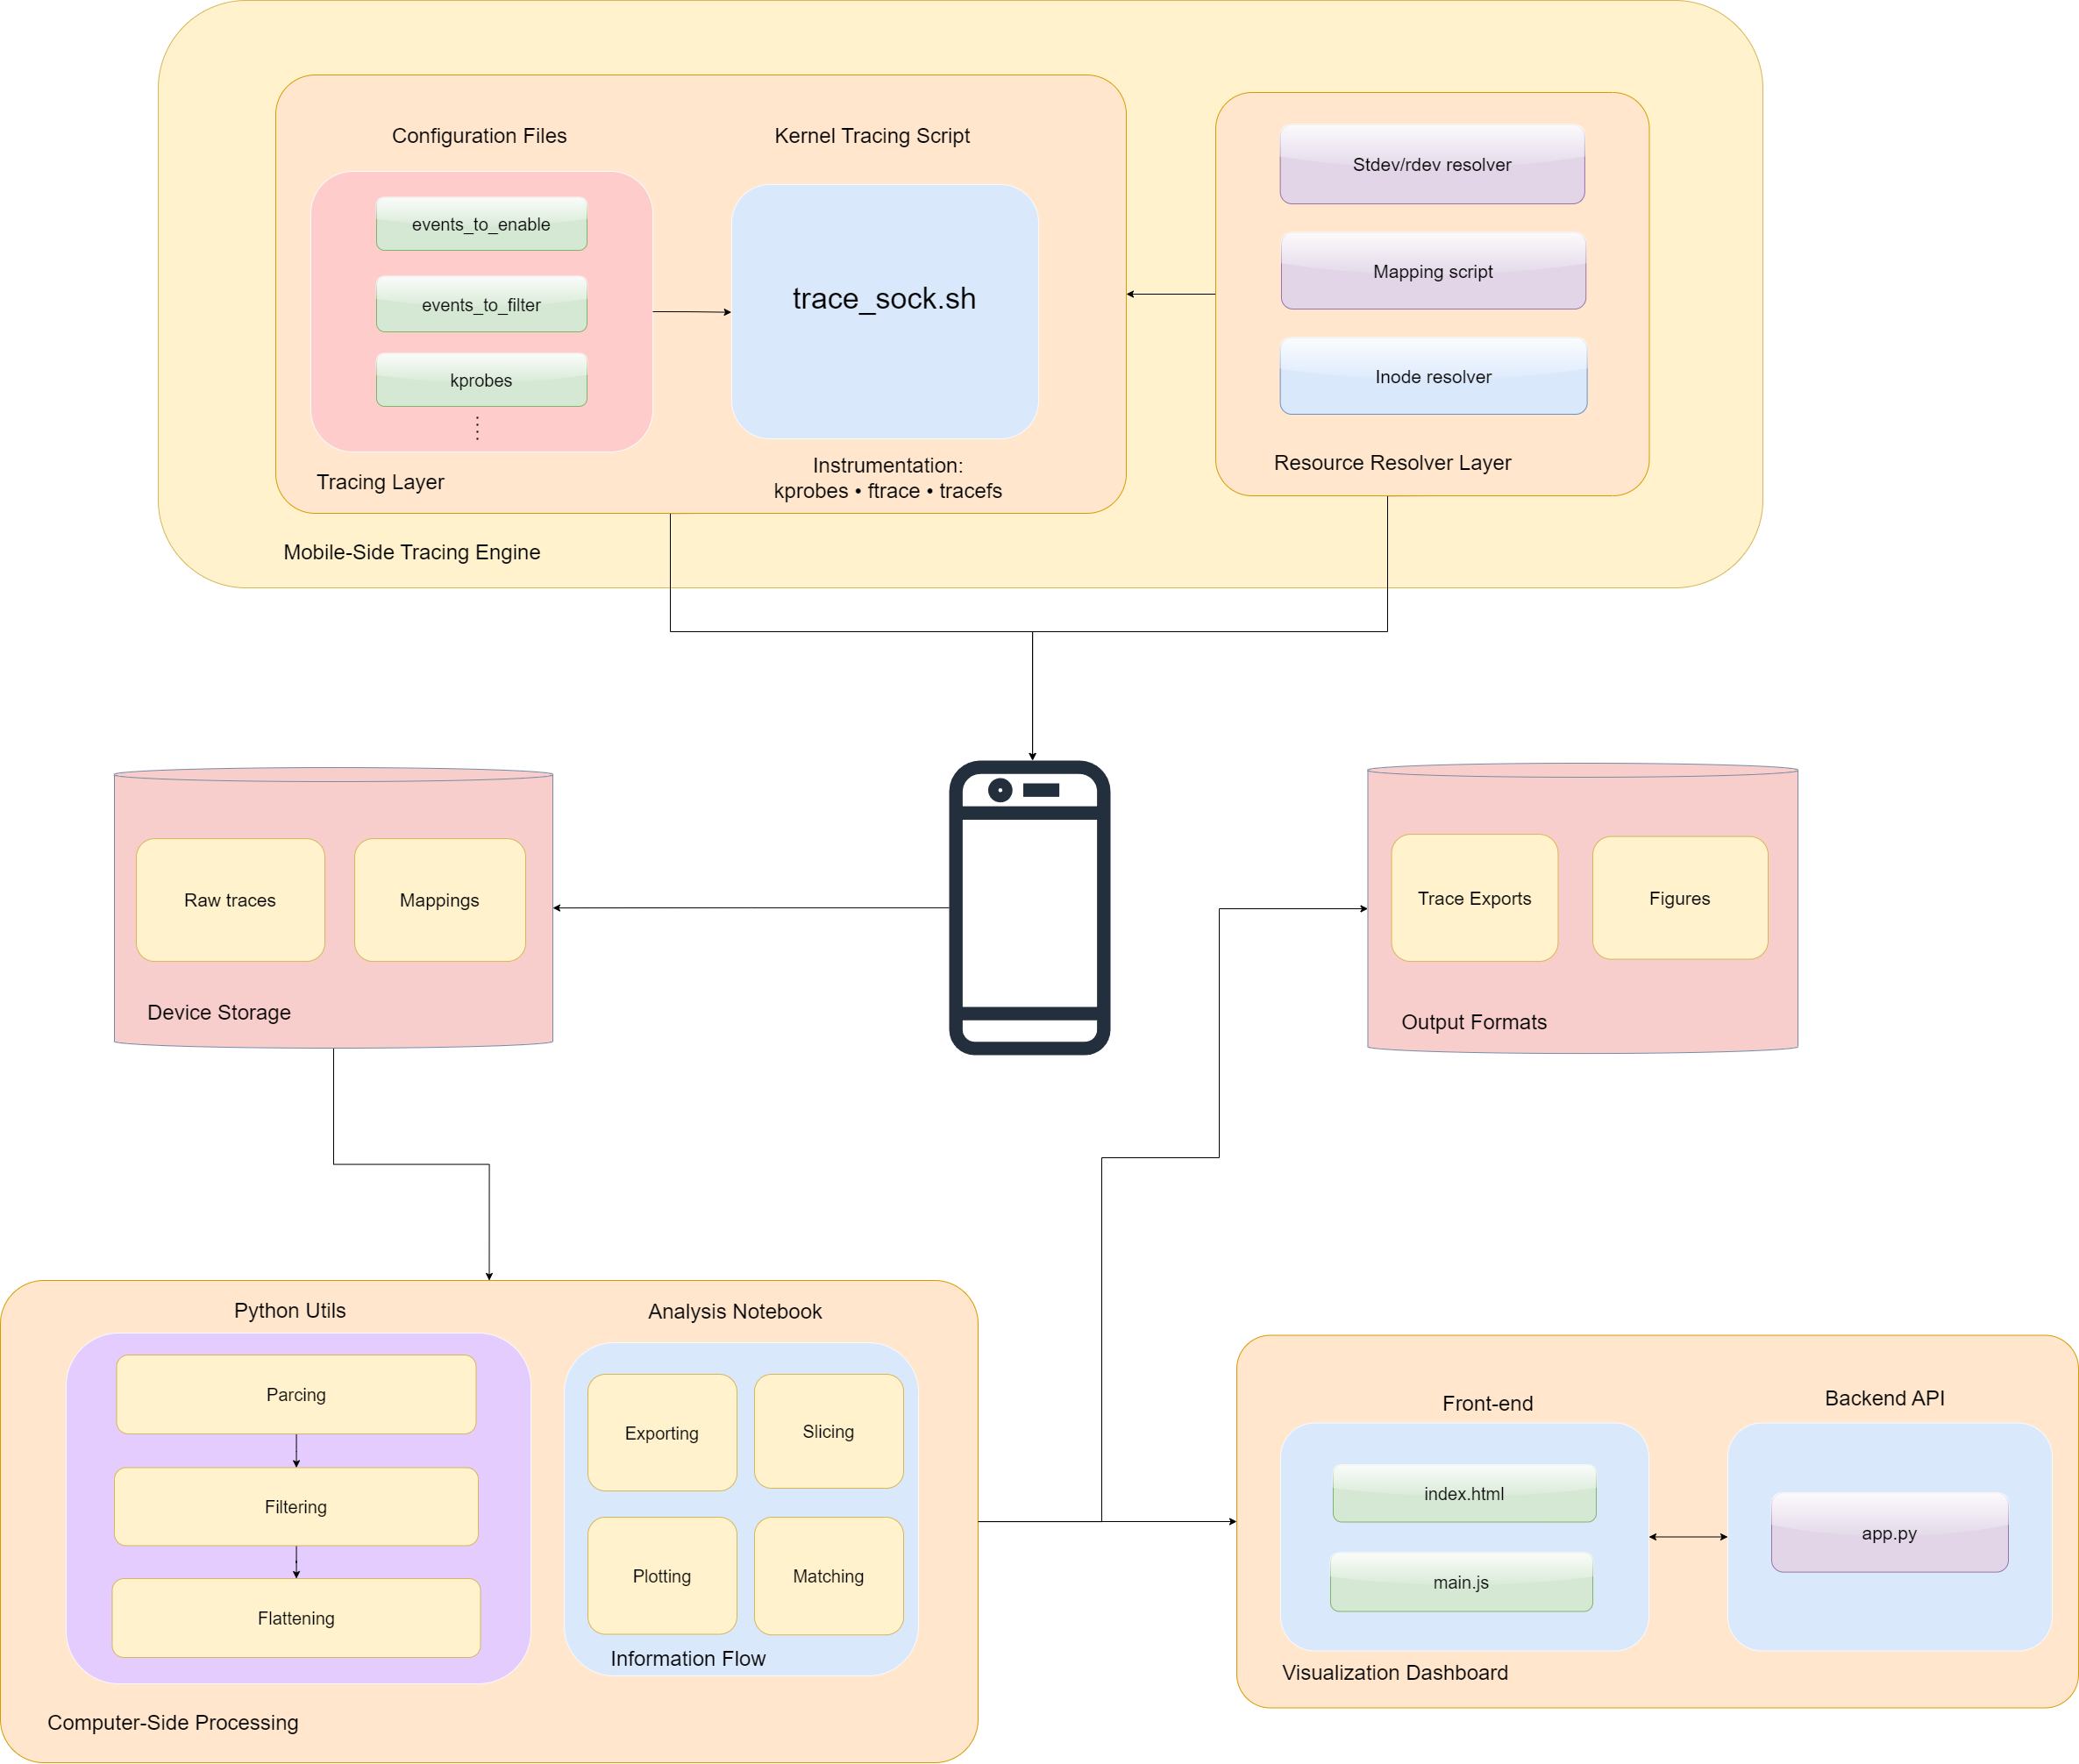
\includegraphics[width=1\textwidth]{architecture.png}
\caption{High-level modular architecture and data-flow pipeline of SliceDroid.}
\label{fig:architecture}
\end{figure}



\subsubsection{Codebase Structure}

The codebase is organised into clearly defined top-level components to support trace collection, processing, and interactive exploration. The main elements are outlined below:

\begin{description}
  \item[\texttt{scripts/}] Contains tracing and resource-mapping scripts. It includes configuration files for enabled events, kprobes, and process filters, as well as helper scripts for resolving device and inode identifiers.

  \item[\texttt{run\_slicedroid.py}] Entry point for running the customised SliceDroid tracer with the specified settings.

  \item[\texttt{data/}] Serves as the central storage for raw traces, identifier mappings, and processed outputs. It includes the \texttt{Exports/} subfolder, which holds cleaned trace exports and generated figures.

  \item[\texttt{webapp/}] Hosts the web-based visualisation tool, with a Flask backend and a Bootstrap/D3.js frontend for displaying behavioural timelines and analytics.
\end{description}

\subsubsection{Instrumentation Layer}

The instrumentation layer is responsible for capturing low-level system interactions occurring on the Android device. The initial implementation of the tracing subsystem was developed by Nikos Alexopoulos as part of the SliceDroid project at AUEB, and forms the foundational backbone of this thesis. This base layer leverages dynamic kernel probes (\texttt{kprobes}) and static \texttt{tracepoints} exposed via the \texttt{ftrace} interface, allowing efficient interception of system call and function-level activity in the kernel.

The original setup includes probes on core I/O functions such as \texttt{vfs\_read}, \texttt{vfs\_write}, and \texttt{do\_vfs\_ioctl}, enabling access to internal kernel structures (e.g., \texttt{file}, \texttt{inode}, \texttt{super\_block}) and extraction of metadata such as device and inode identifiers, file types, and access credentials. In addition, Binder transactions are captured using the static tracepoints \texttt{binder\_transaction} and \texttt{binder\_transaction\_received}.

In the context of this thesis, we extended the instrumentation layer to include additional \texttt{kprobes} targeting network-related operations. Specifically, probes were added on functions such as \texttt{\_\_tcp\_sendmsg}, \texttt{udp\_sendmsg}, \texttt{inet\_sendmsg}, \texttt{sys\_sendto}, \texttt{sys\_bind}, and \texttt{tcp\_connect}, enabling the reconstruction of socket-level behaviors and outbound communication events. This augmentation allows for the detection of privacy-sensitive network transmissions and complements the I/O and IPC tracing pipeline with external data flow visibility.

An example of a \texttt{kprobe} used to trace write operations through the \texttt{vfs\_write} function is shown below:

\begin{lstlisting}[language=bash,caption={Example kprobe for vfs\_write in tracefs syntax}]
p:kprobes/write_probe vfs_write file=$arg1 buf=$arg2 count=$arg3
  inode=+64(+32($arg1)):u64
  k_dev=+76(+32($arg1)):u32
  s_dev=+16(+40(+32($arg1))):u32
  i_mode=+0(+32($arg1)):u16
  kuid=+4(+32($arg1)):u32
  kgid=+8(+32($arg1)):u32
  name=+0(+40(+24($arg1))):string
\end{lstlisting}

Instrumentation is activated through on-device \texttt{bash} scripts, which dynamically configure and manage the tracing session using declarative configuration files. These files specify the enabled probes, filter targets (e.g., process names, syscalls), and logging preferences. All events are timestamped with nanosecond precision to enable accurate temporal correlation during analysis.

This modular instrumentation layer is lightweight, compatible with existing Android kernels, and deployable without kernel recompilation or Android framework modifications. It provides the raw behavioral signal that drives the parsing, slicing, and behavior reconstruction pipeline described in the following sections.


\subsubsection{Resource Resolver Layer}

The \emph{Resource Resolver Layer} bridges the semantic gap between
raw kernel identifiers and human–readable resource categories.  It
accepts two heterogeneous streams that originate from the
Instrumentation Layer:

\begin{enumerate}
  \item \textbf{Special‐device nodes}\,: 32-bit packed
        \texttt{dev\_t} values (\texttt{k\_dev}) extracted from
        \texttt{vfs\_read}/\texttt{vfs\_write}/\texttt{ioctl} probes.
  \item \textbf{Regular files}\,: \texttt{(st\_dev,\;inode)} tuples
        identifying SQLite databases that hold privacy-critical data
        (\texttt{contacts2.db}, \texttt{mmssms.db}, \textit{etc.}).
\end{enumerate}

Its task is to emit a many-to-one mapping
\texttt{\{category $\rightarrow$ [identifiers]\}} where
\texttt{category}~$\in$~\{\textit{camera}, \textit{audio\_in},
\textit{bluetooth}, \textit{gnss}, \textit{nfc},
\textit{contacts}, \textit{sms}, \textit{calllog},
\textit{calendar}\}.
Down-stream modules can then reason about ``use camera’’ or ``read
contacts’’ instead of opaque major/minor numbers.

Algorithm~\ref{alg:resolver} captures the essence of the resolver logic
independently of the concrete implementation language.

\begin{algorithm}[H]
\footnotesize
\caption{Resolve low-level identifiers to high-level categories}
\label{alg:resolver}
\DontPrintSemicolon
\KwIn{$D$ : list of device entries $(\text{name},\ \text{rdev},\ \text{owner},\ \text{group})$\\
\phantom{\KwIn{}}$F$ : list of file entries $(\text{path},\ \text{st\_dev},\ \text{inode})$}
\KwOut{Dictionary $M$ : category $\rightarrow$ list of identifiers}
$M \leftarrow \{\}$
\BlankLine
\ForEach{$(name, rdev, owner, group) \in D$}{
    \uIf{$\texttt{camera} \in name$ \textbf{or} $owner = \texttt{camera}$}{
        $M[\text{camera}] \gets M[\text{camera}] \cup \{rdev\}$
    }
    \uElseIf{$name$ starts with \texttt{pcm} \textbf{and} ends with \texttt{c}}{
        $M[\text{audio\_in}] \gets M[\text{audio\_in}] \cup \{rdev\}$
    }
    \ElseIf{$\texttt{bluetooth} \in name$}{
        $M[\text{bluetooth}] \gets M[\text{bluetooth}] \cup \{rdev\}$
    }
    \ElseIf{$\texttt{nfc} \in name$}{
        $M[\text{nfc}] \gets M[\text{nfc}] \cup \{rdev\}$
    }
    \ElseIf{$\texttt{gps} \in name$ \textbf{or} $\texttt{gnss} \in name$}{
        $M[\text{gnss}] \gets M[\text{gnss}] \cup \{rdev\}$
    }
}
\BlankLine
\ForEach{$(path, dev, ino) \in F$}{
    \uIf{$\texttt{contacts} \in path$}{
        $M[\text{contacts}] \gets M[\text{contacts}] \cup \{(dev, ino)\}$
    }
    \uElseIf{$\texttt{mmssms} \in path$}{
        $M[\text{sms}] \gets M[\text{sms}] \cup \{(dev, ino)\}$
    }
    \uElseIf{$\texttt{calllog} \in path$}{
        $M[\text{calllog}] \gets M[\text{calllog}] \cup \{(dev, ino)\}$
    }
    \uElseIf{$\texttt{calendar} \in path$}{
        $M[\text{calendar}] \gets M[\text{calendar}] \cup \{(dev, ino)\}$
    }
}
\Return{$M$}
\end{algorithm}


\paragraph{Scope within this thesis.}
For the purposes of the present dissertation the creation of
\texttt{cat2\_dev\_*.json} was performed manually and
\emph{once-off}; full automation of the resolver workflow (ADB push,
execution, pull, JSON synthesis) was contributed by collaborating
team-members and therefore falls outside the strict scope of this
thesis.  The layer is nevertheless documented here for completeness
as it supplies essential metadata to the behaviour-reconstruction
pipeline described in the following sections.


\subsubsection{Parsing and Pre-Processing}
After the raw kernel traces were collected from the device, they were quickly pre-processed using a lightweight Python parser. Each trace line was split using regular expressions to extract the main header fields (task, PID, CPU, flags, timestamp, event name) and the detailed key-value pairs. Numerical fields were converted to plain decimal form, flags were normalized, and paths were cleaned of extra characters.

Next, a sequence of basic filters removed background noise: well-known system daemons were excluded, short-lived file descriptors were ignored, and redundant Binder transaction chatter was collapsed. Finally, the cleaned trace events were divided into overlapping windows to enable manageable and context-preserving analysis in the next steps. This simplified approach followed the same principles as in SliceDroid but was adapted for faster exploratory profiling.

\subsubsection{Slicing and Information-Flow Tracking}

For each window and seed PID $p$, we reconstruct per-process
information flows using the dual-pass IPC slicing algorithm adapted
from SliceDroid (Algorithms 1–2):

\begin{enumerate}
  \item \textbf{Forward slice (out-flows).}
        Scan events in chronological order; maintain a dynamic set
        $P$ of “reachable’’ PIDs (initially $\{p\}$).
        \emph{IPC $\rightarrow$} events add the destination PID to $P$;
        \emph{write/ioctl/net-send} events emitted by any
        $q\!\in\!P$ are recorded as outward dataflows.
  \item \textbf{Backward slice (in-flows).}
        Repeat in reverse time order; \emph{IPC~$\rightarrow$} adds
        the source PID, and \emph{read/net-recv} events supply the
        inbound dependencies.
\end{enumerate}

Each slice yields a directed, per-window causal graph
$G=(V,E)$ where
$V$ = PIDs and $E$ = \{read, write, ioctl, socket, binder\}.
Graphs are merged across consecutive windows via identical
transaction IDs (Binder) and socket tuples, producing a
whole-session trace of:

\[
  \text{API call} \;\xrightarrow{\;G\;}\;
  \Bigl\{\,
     \text{device nodes},\;
     \text{files},\;
     \text{sockets}
  \Bigr\}
\]

\noindent
The resulting flow descriptors are serialised to
\texttt{JSON/CSV} for downstream analytics and drive both the static
PDF plots and the interactive Flask–D3 dashboard.


\subsection{Data Visualization and User Interface Design}

The SliceDroid platform has been significantly extended into a fully-featured web application with an integrated dashboard, while maintaining its thoughtfully designed, step-by-step interface that guides analysts from initial trace file upload through to detailed security insights and forensics.

Figure~\ref{fig:home_screen} shows the home screen, which acts as the starting point for each analysis session. Users can upload a new raw \texttt{.trace} file by dragging it onto the upload area or selecting it manually. For convenience, the system also supports preloading the most recently used trace file, indicated as \texttt{trace.trace}, so that repeated uploads are not necessary during iterative investigations. In parallel, the user can choose which specific application’s behaviour to examine from a curated list of popular apps (e.g., Messenger, Signal, Telegram, Termux), ensuring that only relevant events are shown in the analysis views. Additional process ID and device filters refine the scope even further before launching the analysis.

\begin{figure}[H]
\centering
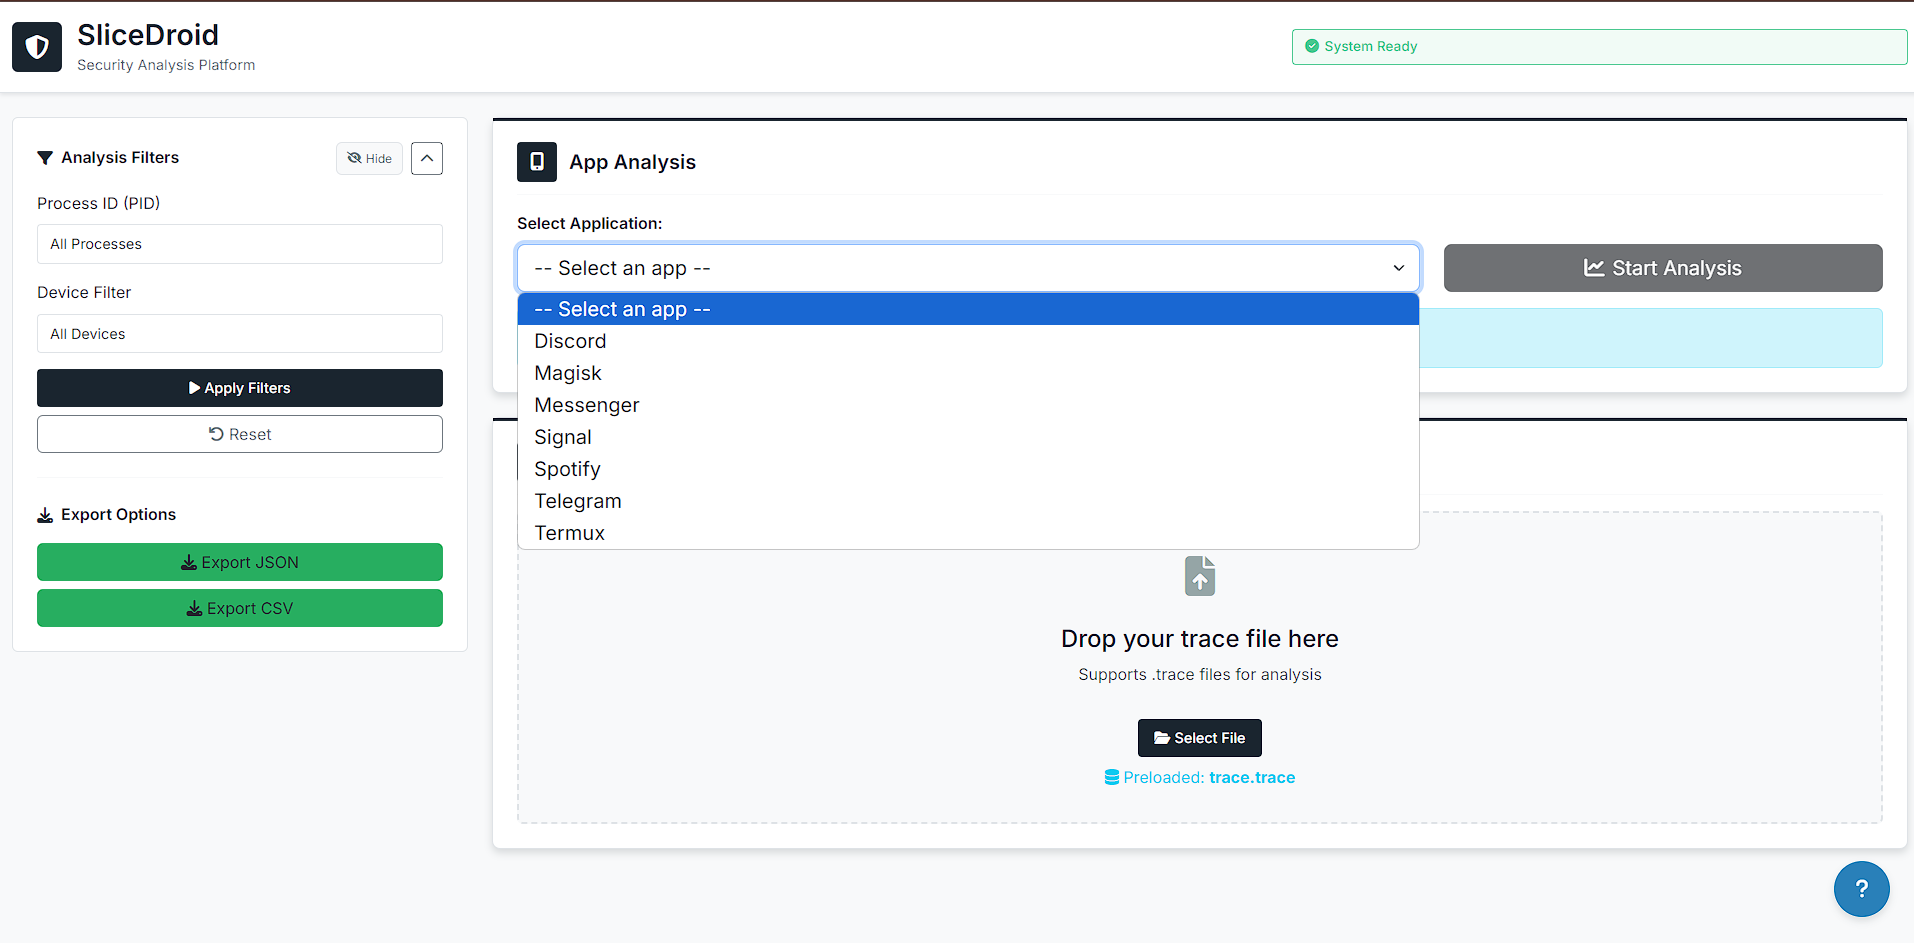
\includegraphics[width=0.95\textwidth]{home_screen.png}
\caption{Home screen with options for uploading a new trace file, preloading the last trace, and selecting a target application for focused security analysis.}
\label{fig:home_screen}
\end{figure}

After selecting the trace and target application, the analyst transitions to the interactive event timeline (Figure~\ref{fig:event_timeline}). This timeline provides a clear, category-separated view of syscall activity over time, grouped into logical classes such as \texttt{read}, \texttt{write}, \texttt{ioctl}, Binder events, and network operations. The timeline supports zooming, panning, and detailed inspection via hover tooltips, allowing investigators to pinpoint unusual spikes, suspicious sequences, or gaps in expected process behaviour.

\begin{figure}[H]
\centering
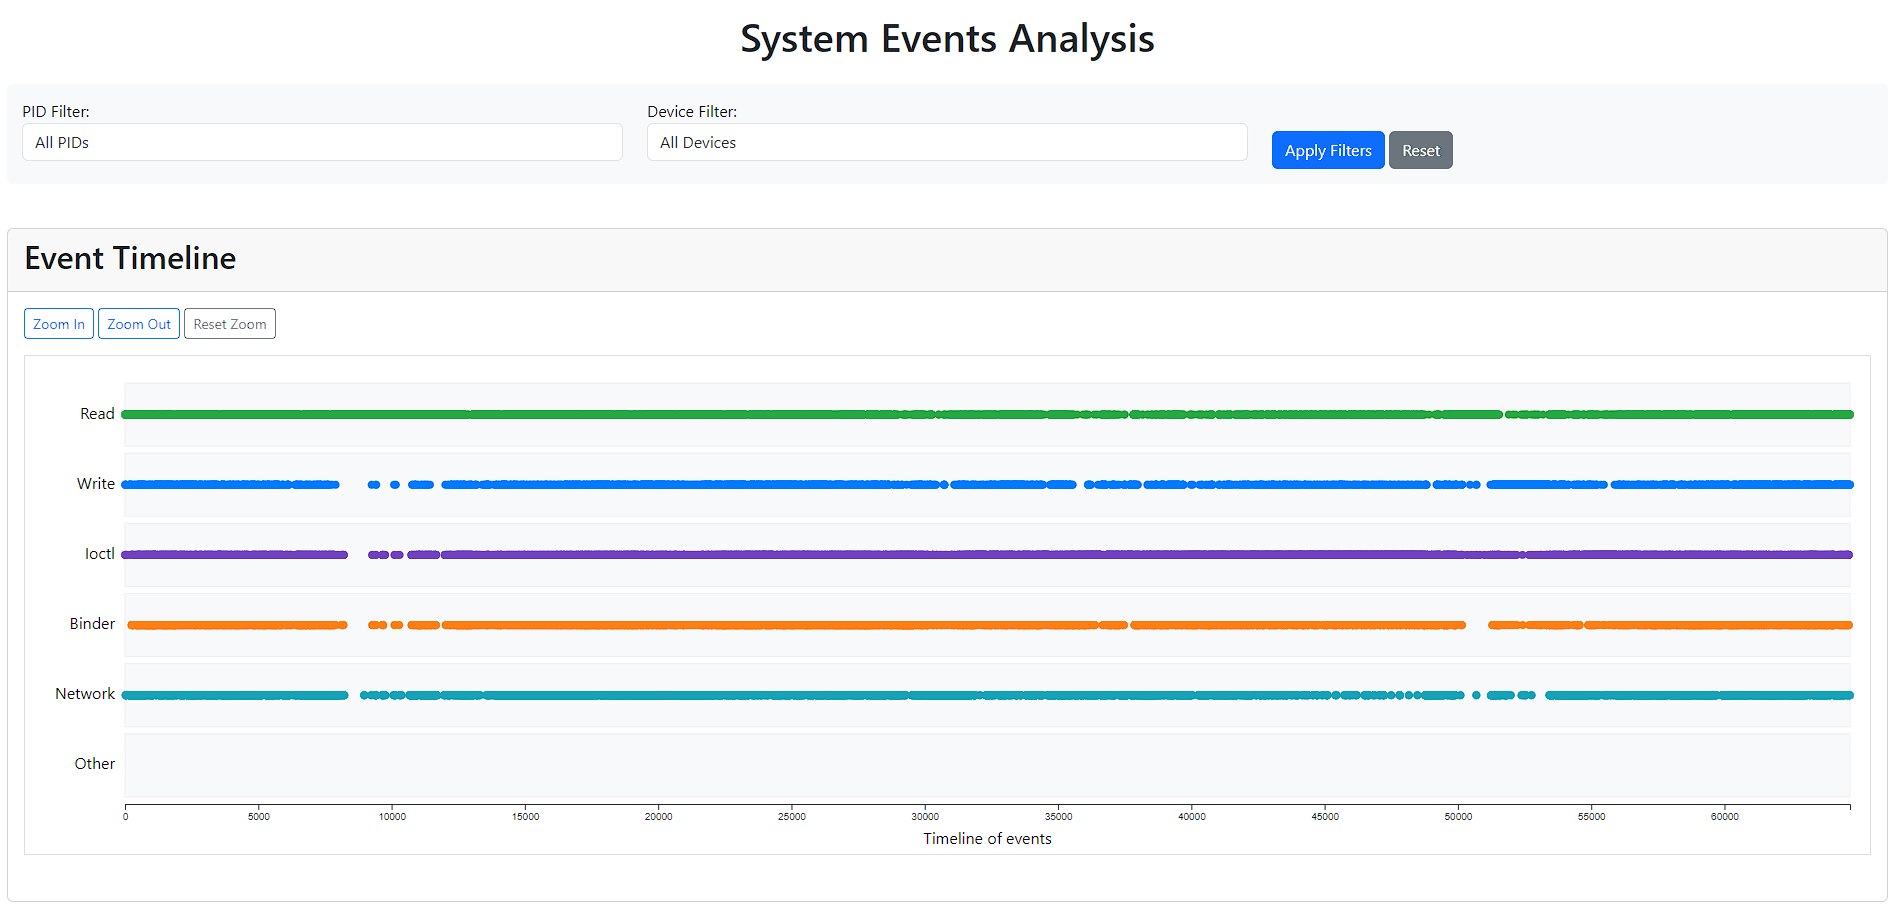
\includegraphics[width=0.95\textwidth]{system_events_timeline.png}
\caption{Interactive event timeline showing syscall activity split into categories with intuitive zoom and hover inspection tools.}
\label{fig:event_timeline}
\end{figure}

Complementary to the timeline is the Device and Event Statistics panel (Figure~\ref{fig:device_event_statistics}). On the left, a pie chart and table break down which hardware devices were accessed during the trace period, highlighting the top devices by event count. On the right, the system shows the proportion of syscall event types (e.g., \texttt{ioctl\_probe}, \texttt{read\_probe}), their absolute counts, and percentage shares. This dual view helps analysts understand which resources and syscall classes dominate the workload, which is often critical for detecting outlier device usage or unexpected access patterns.

\begin{figure}[H]
\centering
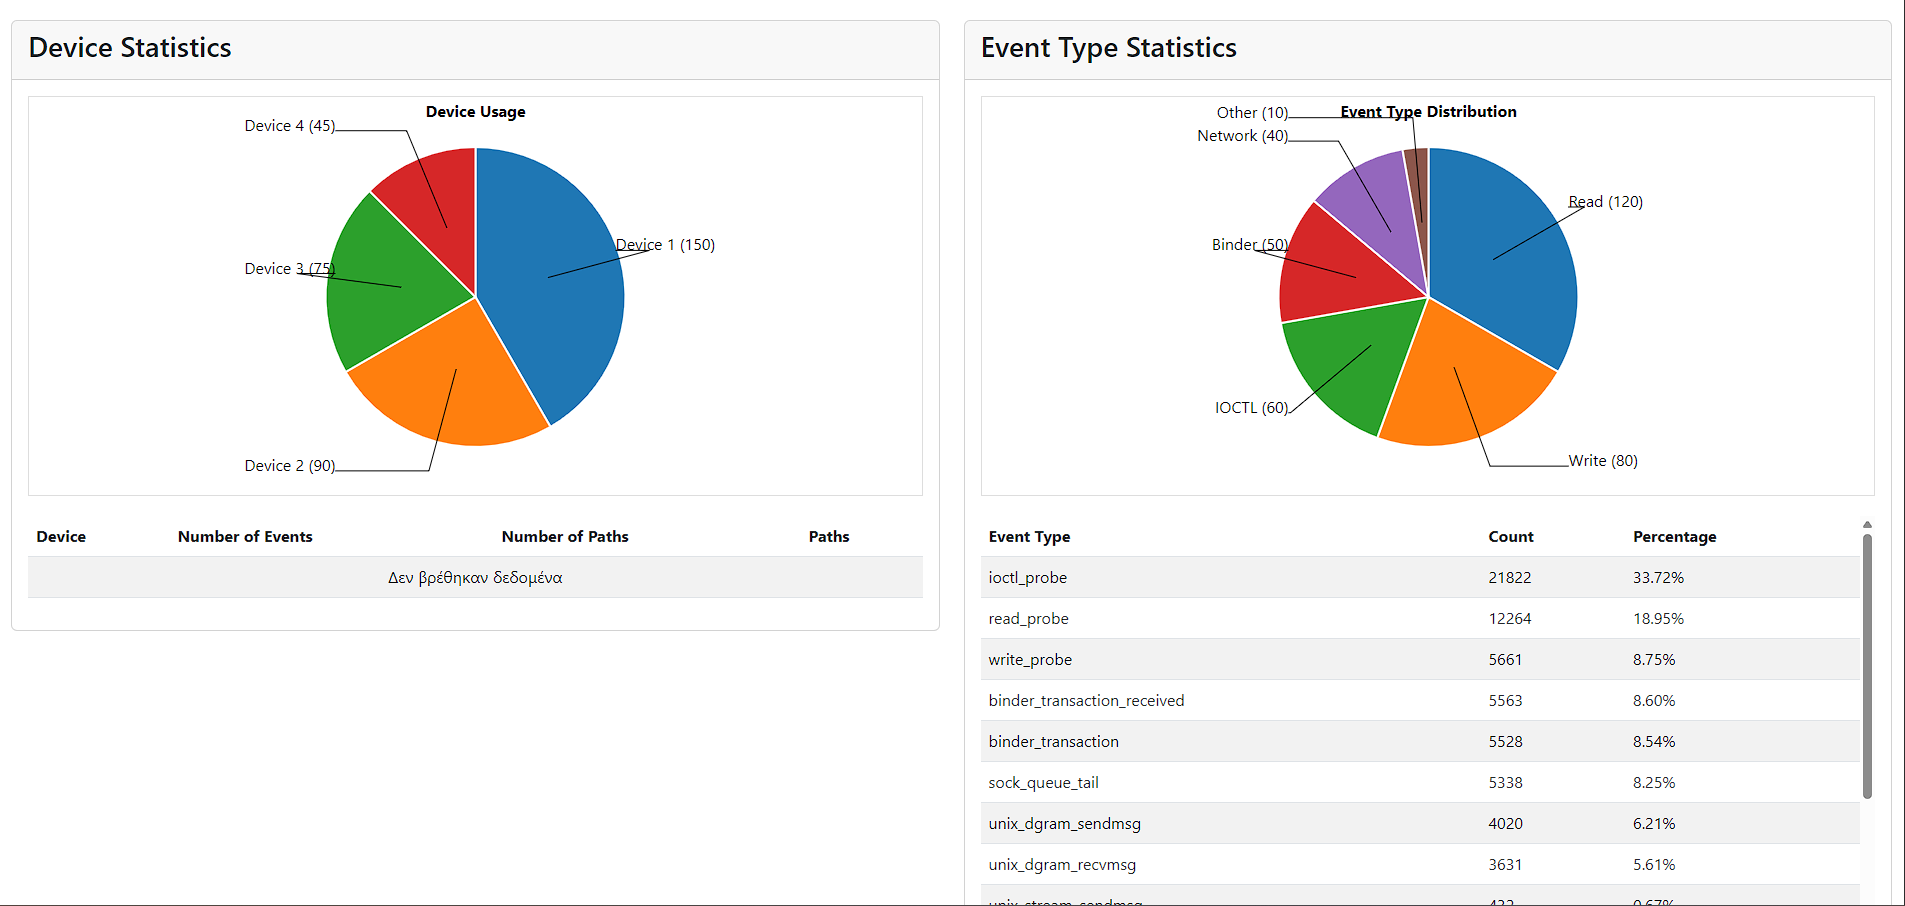
\includegraphics[width=0.95\textwidth]{device_event_statistics.png}
\caption{Device and event statistics: left pane shows device usage distribution and top devices; right pane displays breakdown of syscall event types.}
\label{fig:device_event_statistics}
\end{figure}

Figure~\ref{fig:analytics_panel} presents the Advanced Analytics module. This section displays high-level metrics including total event count, unique processes and devices, trace duration, and calculated event throughput in events per second. Below these KPIs, the Behaviour Timeline plots activity windows for categories like Camera, TCP, Bluetooth, SMS, and other sensitive subsystems. This windowed view helps correlate spikes in device behaviour with specific time windows, enabling fine-grained behavioural profiling.

\begin{figure}[H]
\centering
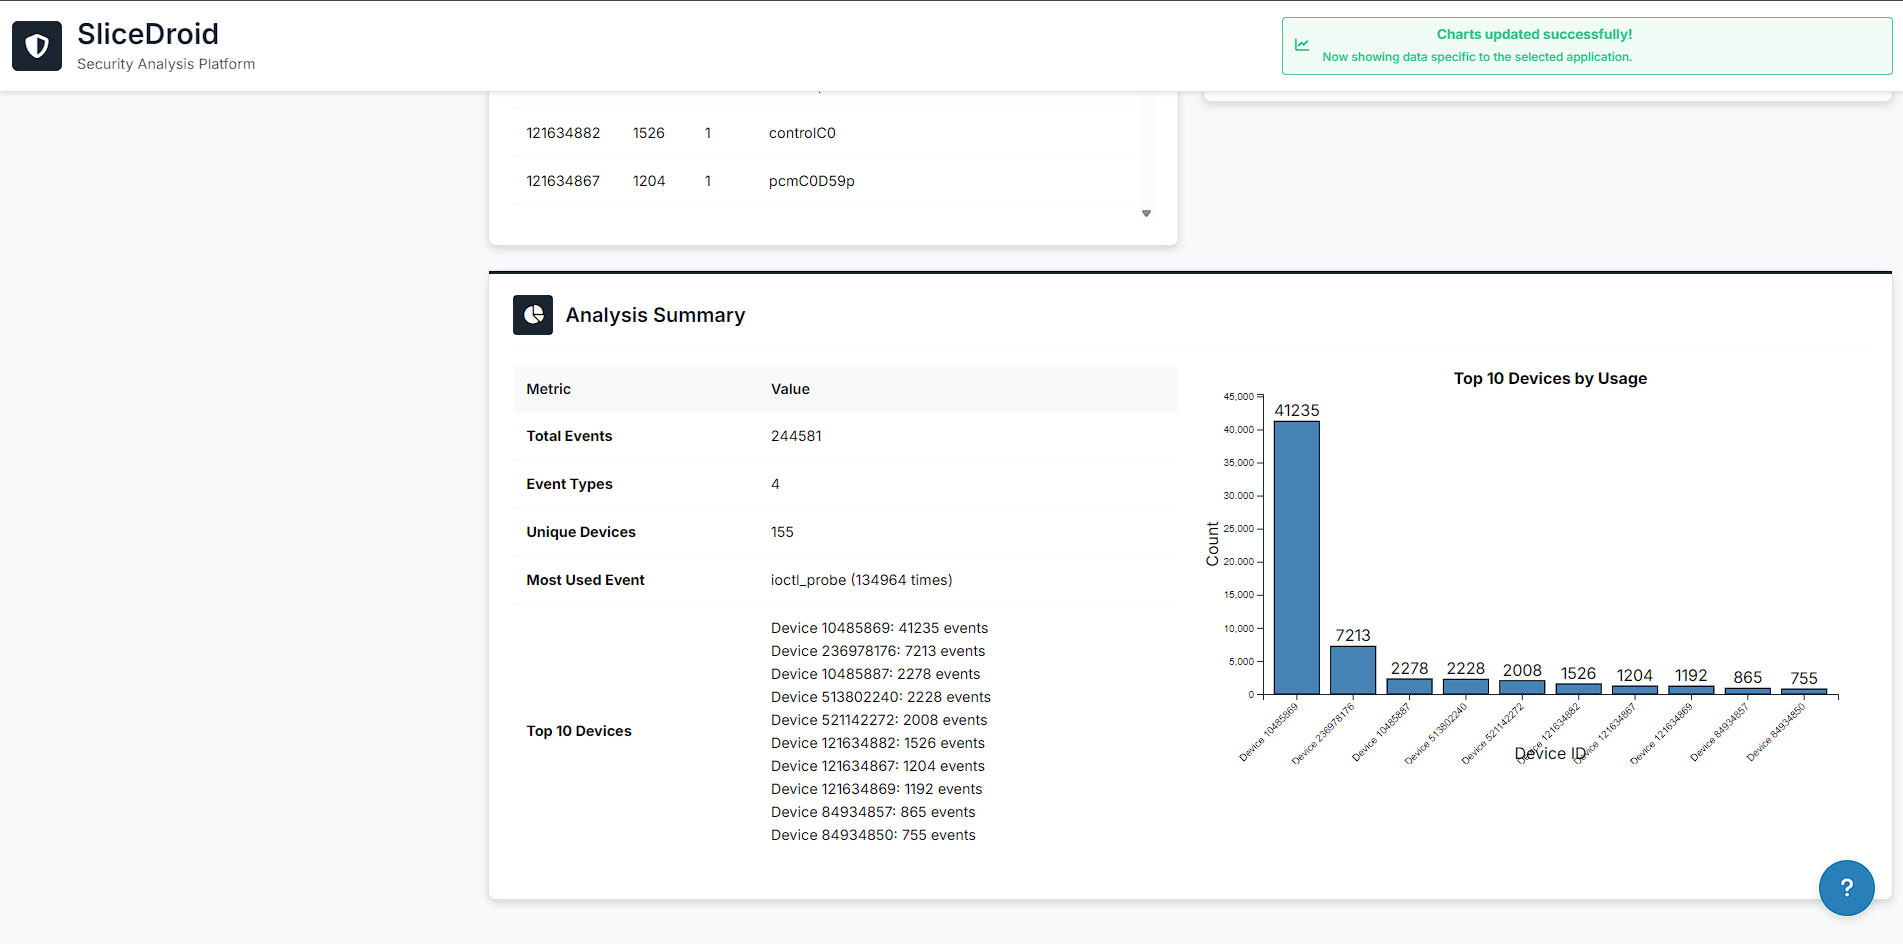
\includegraphics[width=0.95\textwidth]{analytics_panel.png}
\caption{Advanced Analytics: high-level metrics and the Behaviour Timeline, offering windowed insight into sensitive categories such as network and peripheral usage.}
\label{fig:analytics_panel}
\end{figure}

For focused inspection of network behaviour, the Network Analysis module (Figure~\ref{fig:network_view}) visualises the distribution of TCP and UDP events, socket operations, and the protocols in use. A graph-based Communication Flow diagram depicts the relationships between processes and external endpoints. Such visual context allows the investigator to detect unexpected data transfers or suspicious inter-process communication pathways.

\begin{figure}[H]
\centering
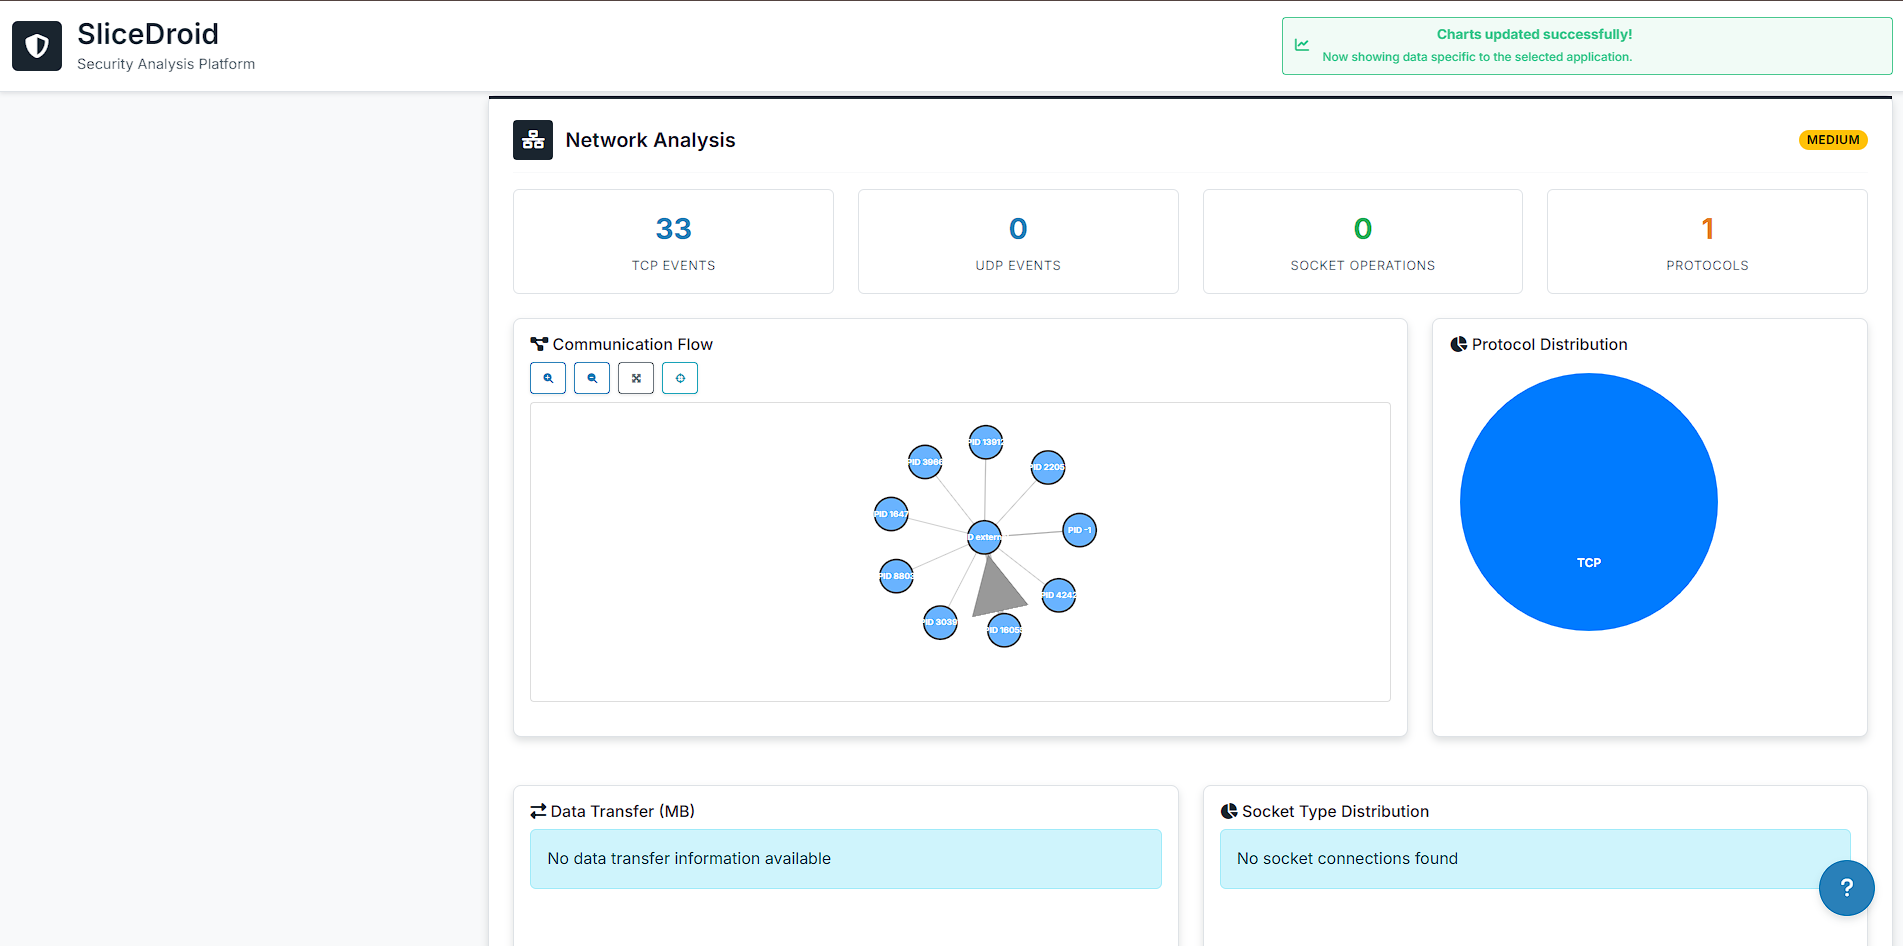
\includegraphics[width=0.95\textwidth]{network_view.png}
\caption{Network Analysis: Communication Flow diagram, protocol distribution pie chart, and connection statistics for tracking network behaviour and potential exfiltration vectors.}
\label{fig:network_view}
\end{figure}

Process genealogy is equally crucial. Figure~\ref{fig:process_tree} illustrates how the system reconstructs the parent-child process tree, showing process activity summaries including PIDs, event counts, and suspicious patterns (highlighted below the tree). Here, anomalies such as excessive file accesses or unexpected forks can be quickly identified and traced back to their origin.

\begin{figure}[H]
\centering
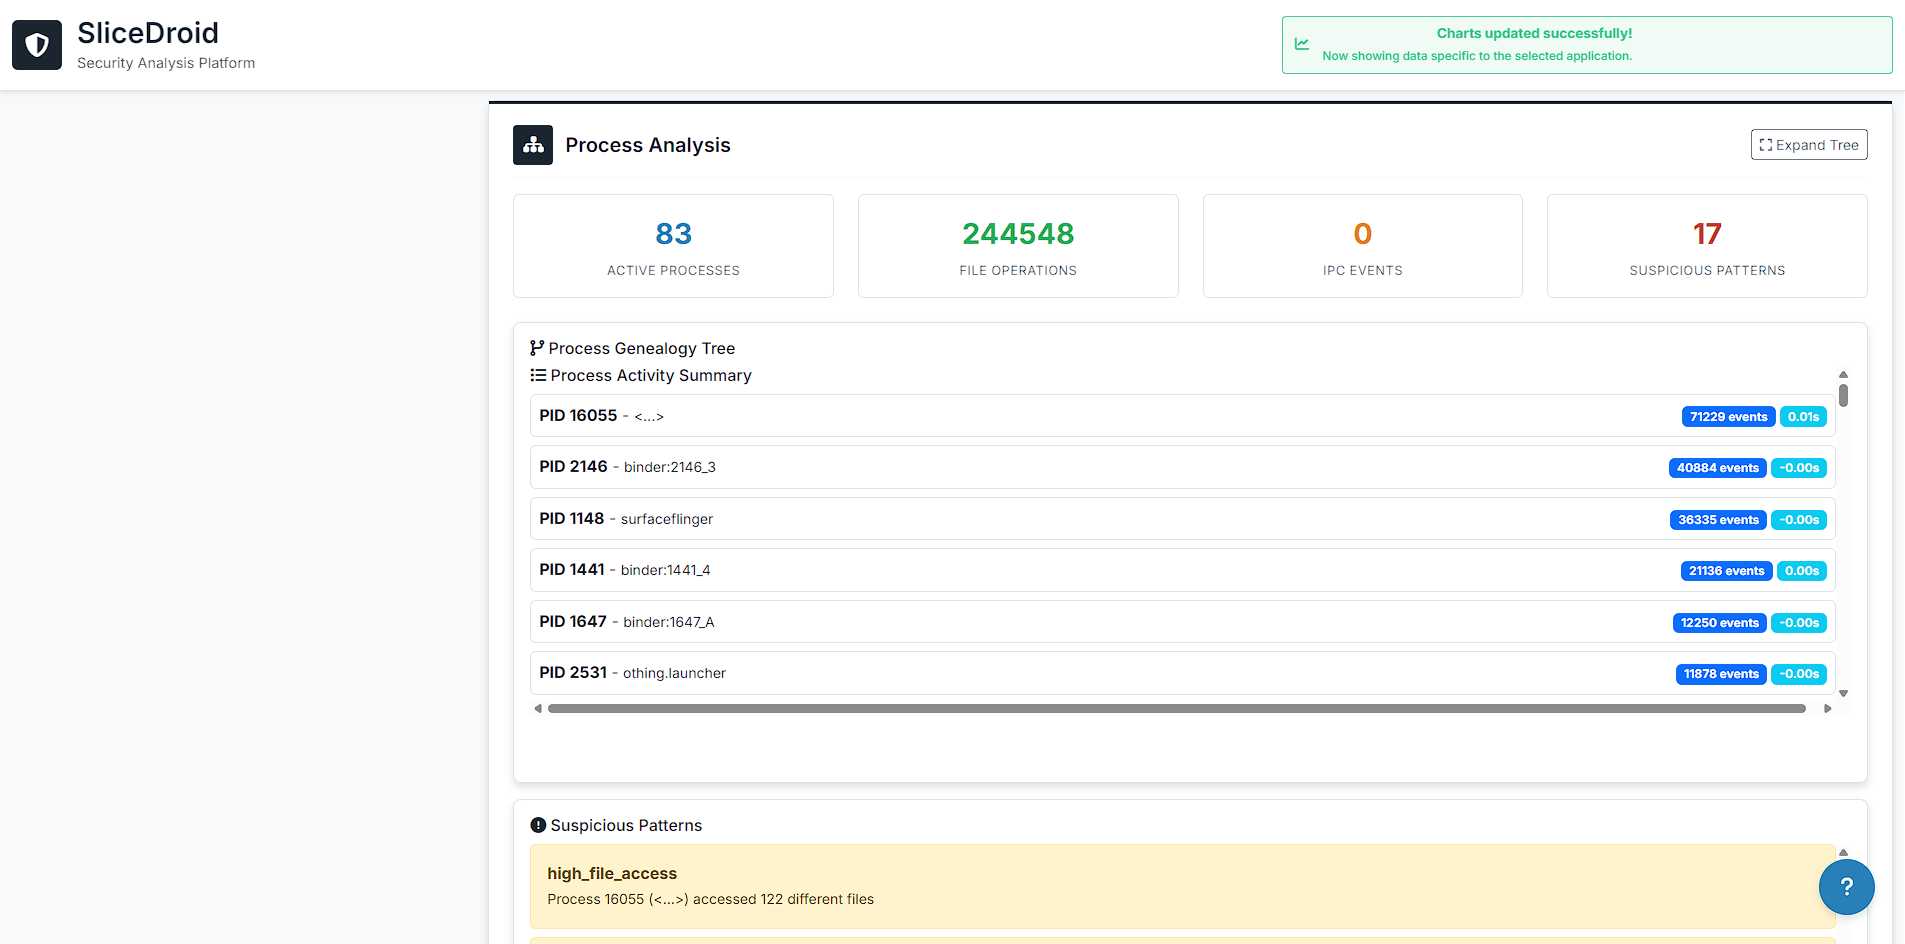
\includegraphics[width=0.95\textwidth]{process_tree.png}
\caption{Process Analysis: dynamic genealogy tree with activity summary and detected suspicious patterns, such as high file access counts.}
\label{fig:process_tree}
\end{figure}

Finally, Figure~\ref{fig:security_overview} shows the dashboard’s integrated security summary. This view aggregates risk scores, highlights privilege escalation attempts, debugging traces, or policy violations, and provides contextual recommendations for remediation. By centralising these indicators, analysts can prioritise threats and document findings more effectively.

\begin{figure}[H]
\centering
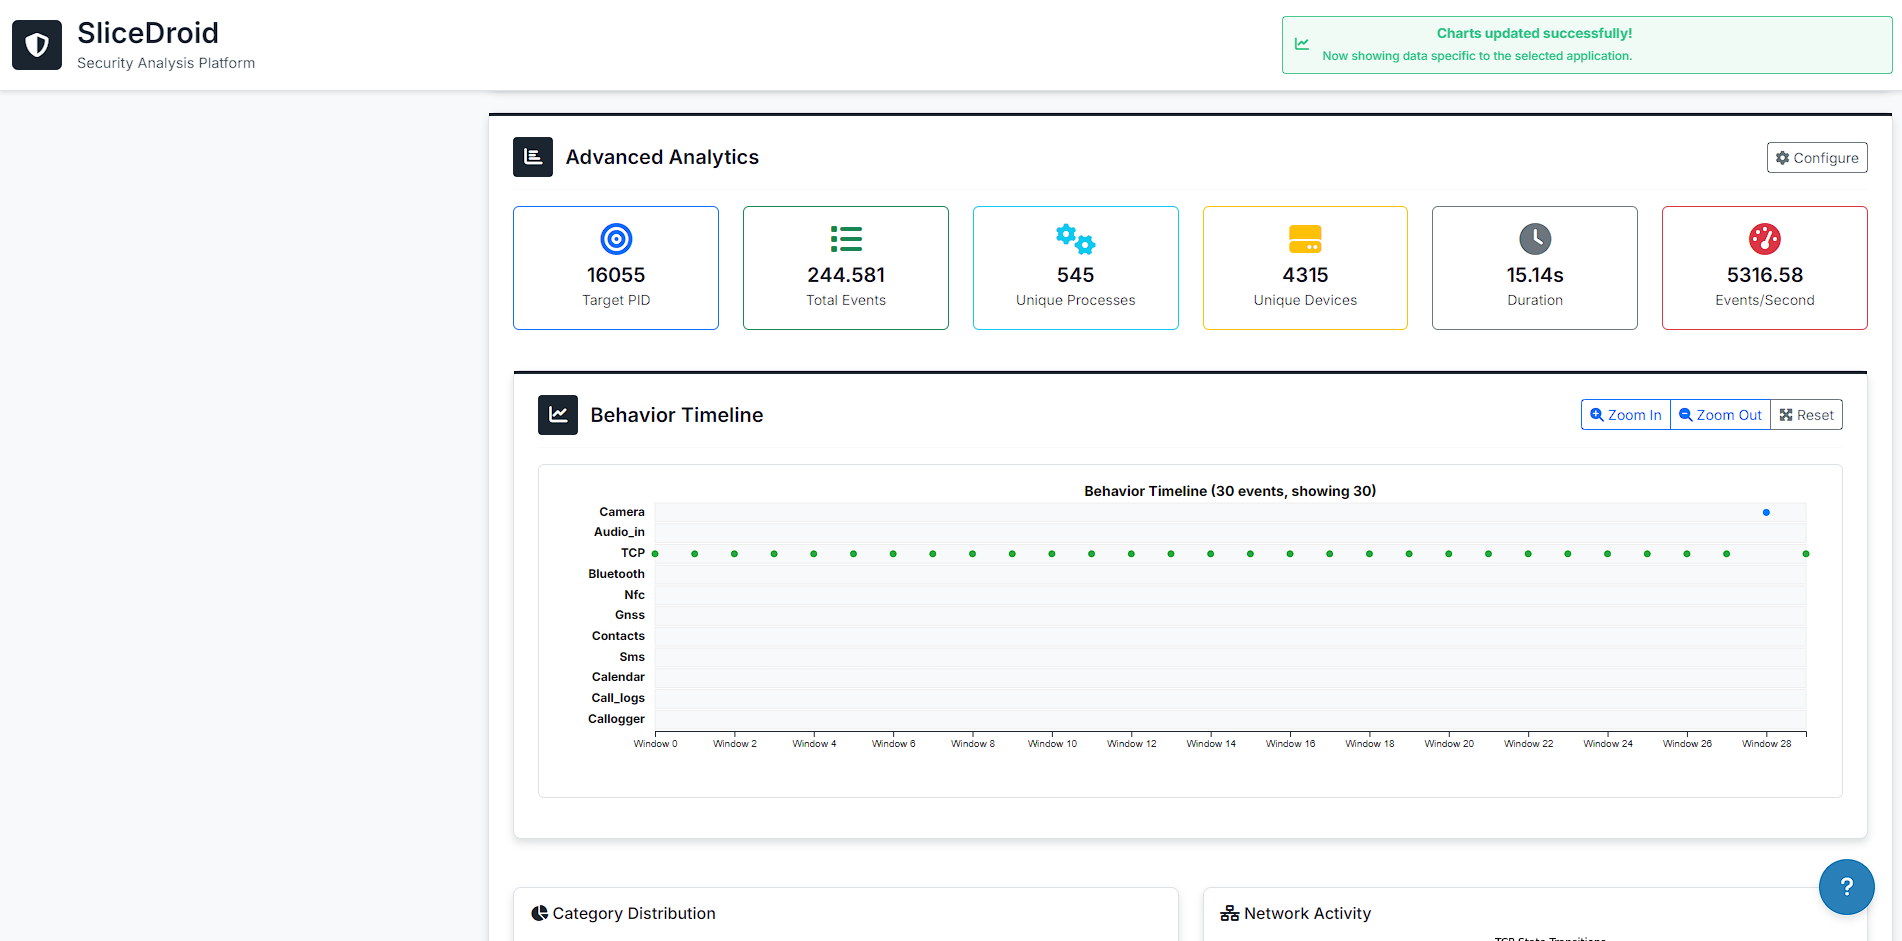
\includegraphics[width=0.95\textwidth]{security_overview.png}
\caption{Security Overview: centralised display of detected risks, privilege escalation attempts, and recommended actions for the analyst.}
\label{fig:security_overview}
\end{figure}

In summary, the combined views — including the timeline, device and event statistics, advanced analytics, network and process modules, and security overlays — converge in a comprehensive summary dashboard (Figure~\ref{fig:summary_dashboard}). This final snapshot condenses category distribution, TCP state transitions, top device usage, and most active processes into a single, intuitive screen, offering a clear, actionable overview for immediate security insight and reporting.

\begin{figure}[H]
\centering
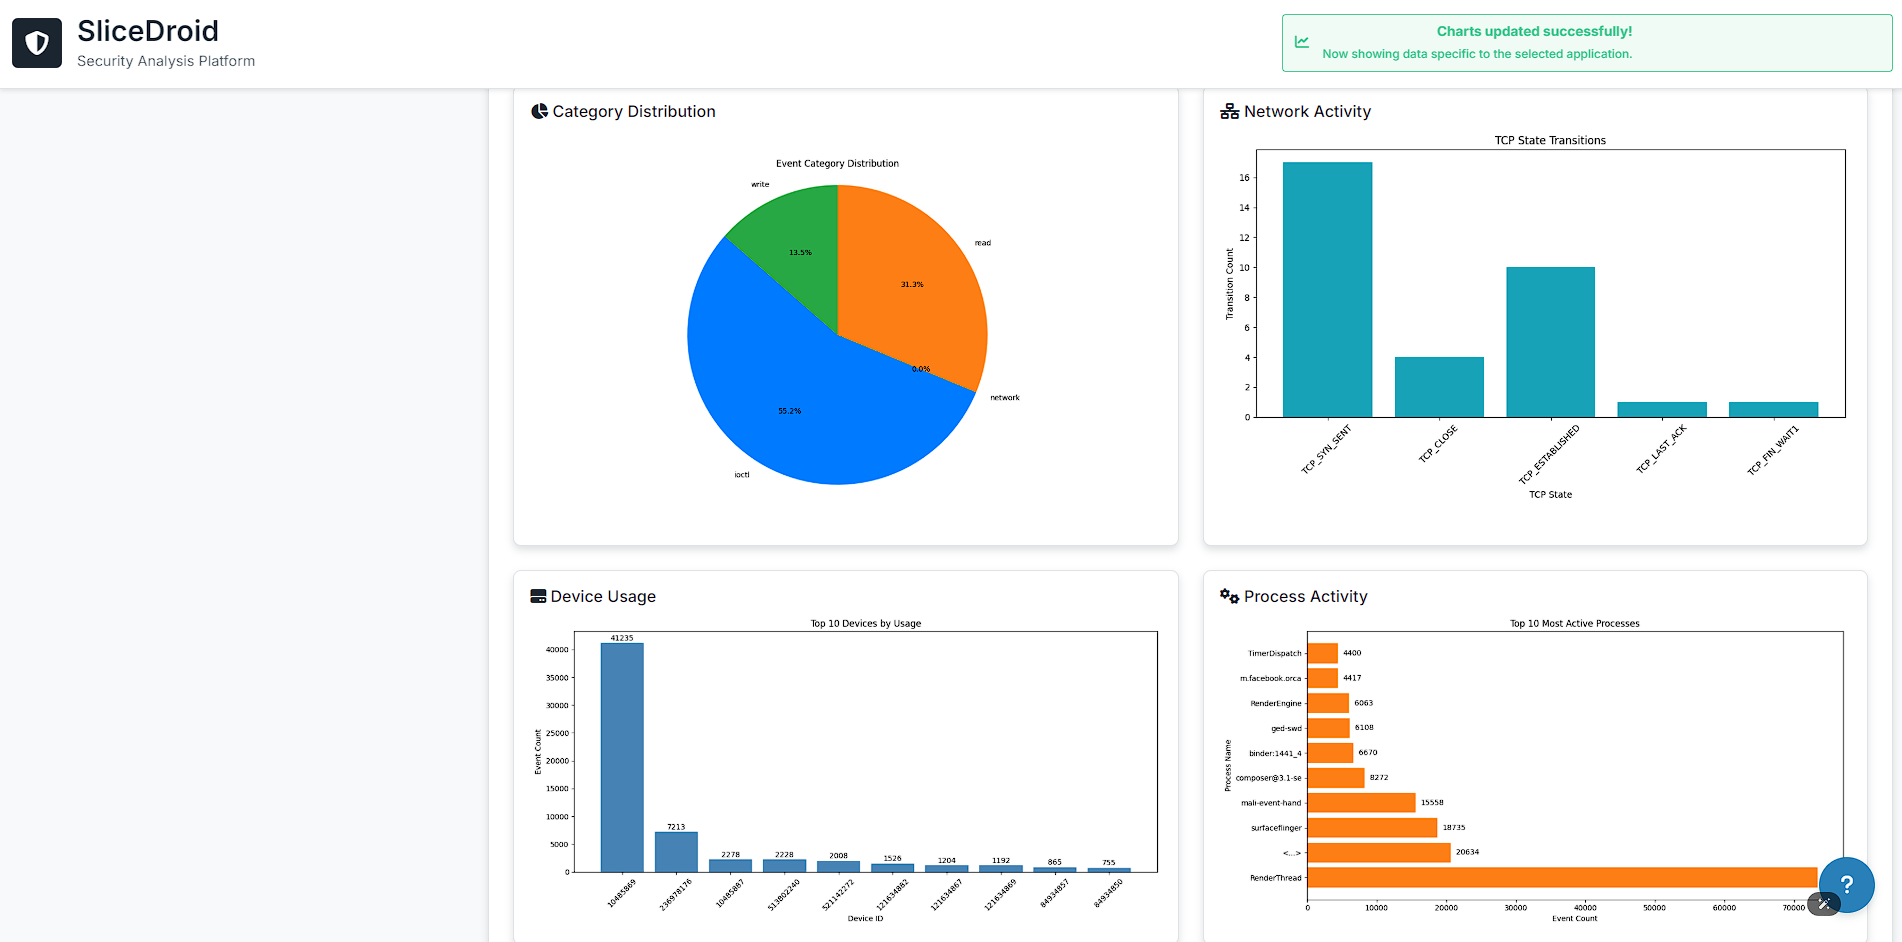
\includegraphics[width=0.95\textwidth]{security_overview-2.png.png}
\caption{Comprehensive Summary Dashboard: unified visual of event categories, TCP states, device usage, and active process distribution for rapid situational awareness.}
\label{fig:summary_dashboard}
\end{figure}

Technically, all dynamic charts are rendered using \texttt{D3.js}, and the responsive UI is built with \texttt{Bootstrap}. A collapsible sidebar, integrated help tooltips, and live system health checks ensure usability and reliability throughout long-duration trace analysis sessions.

\subsubsection{Pipeline Summary}

To close this architecture chapter, Figure \ref{fig:pipeline} condenses the entire workflow into eight blocks: configuration and probe activation, low-overhead collection via \texttt{tracefs}, host-side parsing, cleaning, IPC slicing, export, a Flask API, and finally a D3.js dashboard.  Each block is self-contained, so downstream components can be swapped without touching the upstream instrumentation layer.

\begin{figure}[H]
\centering
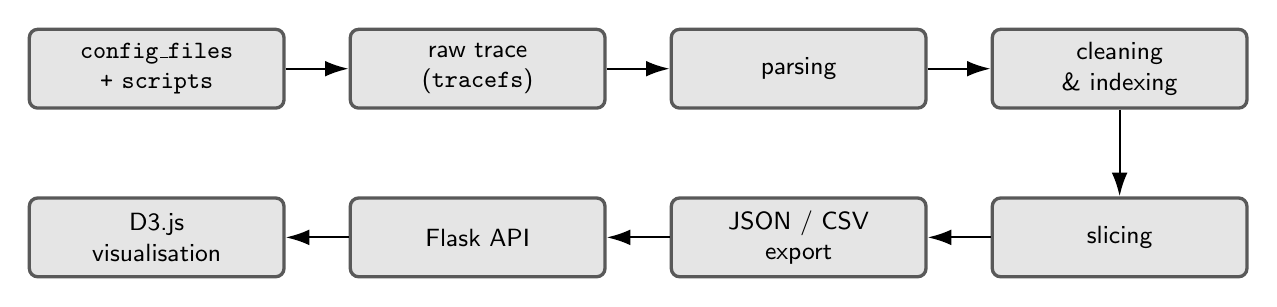
\begin{tikzpicture}[
  font=\sffamily\small,
  box/.style={
     rectangle, rounded corners=3pt,
     draw=black!65, very thick,
     fill=gray!20,
     text width=3cm, align=center,
     minimum height=1.0cm},
  arrow/.style={-{Latex[length=3mm,width=2mm]}, thick},
  node distance=1.3cm and 0.8cm]
% first row
\node[box] (cfg)   {\texttt{config\_files}\\\texttt{+ scripts}};
\node[box,right=of cfg]  (raw)   {raw trace\\(\texttt{tracefs})};
\node[box,right=of raw]  (parse) {parsing};
\node[box,right=of parse] (clean) {cleaning\\\& indexing};
% second row
\node[box,below=1.1cm of clean] (slice) {slicing};
\node[box,left=of slice]        (exp)   {JSON / CSV\\export};
\node[box,left=of exp]          (api)   {Flask API};
\node[box,left=of api]          (viz)   {D3.js\\visualisation};
% arrows
\path[arrow]
  (cfg) edge (raw)
  (raw) edge (parse)
  (parse) edge (clean)
  (clean) edge[below] (slice)
  (slice) edge (exp)
  (exp) edge (api)
  (api) edge (viz);
\end{tikzpicture}
\caption{End-to-end data flow from probe configuration to interactive analytics.}
\label{fig:pipeline}
\end{figure}

\subsection{Workload Design and Usage Scenarios}

To capture meaningful behavioural variations and to systematically compare how each application responds under distinct runtime conditions, dynamic kernel-level tracing was organised into four carefully defined usage scenarios per target app. This multi-scenario design enables direct cross-scenario comparison, revealing differences in resource usage, inter-process communication (IPC), and network interactions when permissions or user activity levels vary.

\begin{enumerate}[label=\roman*.]
  \item \textbf{Full Permissions Scenario:} The application was run with all permissions granted, allowing observation of its maximum functional scope. In this mode, a consistent sequence of actions was performed: sending two text messages, recording a short voice message (approximately 5 seconds long), and capturing a photo using the in-app camera. This interaction pattern ensures coverage of typical real-world usage and tests multiple privacy-sensitive features simultaneously. The full permissions scenario serves as a baseline to compare against restricted and passive states, helping isolate which activities depend on specific permissions.

  \item \textbf{Restricted Permissions Scenario:} Selected sensitive permissions (e.g., location, microphone, or contacts) were deliberately disabled through the Android settings. This condition was designed to examine how the application adapts when permission-dependent features are blocked—whether it attempts repeated access, triggers fallback code, or suppresses functionality altogether. Comparing this scenario to the full permissions case highlights how gracefully or aggressively each app handles denied permissions.

  \item \textbf{Background Passive Scenario:} The app was left running in the background with normal permissions but without user interaction. This scenario was included to detect silent background behaviours such as periodic syncs, push notification handling, or unexpected network calls that occur independently of user input. Analysing this passive state alongside active usage reveals latent behaviours that could impact privacy or battery consumption.

  \item \textbf{Active Foreground Scenario:} The app was actively used for normal tasks such as messaging, media sharing, and voice or video calls where applicable. This scenario represents the peak operational state with frequent user actions, providing a reference for typical real-world usage patterns. Comparing it with the passive and restricted runs helps pinpoint which kernel-level events are triggered exclusively by user-initiated activity versus background processes.
\end{enumerate}

Each scenario execution lasted approximately one minute to capture sufficient behavioural samples and was repeated multiple times to enhance reliability and minimise outlier effects. The runs were systematically scheduled in a consistent sequence—starting from passive, followed by restricted, then full permissions, and concluding with active usage—to ensure stable device conditions and to avoid cross-contamination of residual states.

By applying this structured workload design, the resulting traces enable detailed side-by-side comparisons. This makes it possible to clearly identify behavioural deviations across permission settings and activity states, providing deeper insights into each application's runtime privacy implications and resource footprint.


% --------------------------------------------------
%  Results
% --------------------------------------------------
\chapter{Results}

\section{Static Analysis Results}

This chapter presents a detailed \emph{static} security appraisal of three widely used instant messaging clients—\textit{Signal}, \textit{Telegram}, and \textit{Meta Messenger}—based on production-signed APK packages acquired directly from physical Android devices using the ADB. Specifically, each APK was retrieved via the following commands:

First, all installed packages on the device were enumerated with:
\begin{lstlisting}[language=bash]
adb shell pm list packages
\end{lstlisting}

Next, the full installation path of a selected package was queried:
\begin{lstlisting}[language=bash]
adb shell pm path <package_name>
\end{lstlisting}

Finally, the APK was pulled to the local workstation:
\begin{lstlisting}[language=bash]
adb pull /data/app/<apk_path> ./
\end{lstlisting}

The subsequent static evaluation utilises tools including \textsc{MobSF}, \textsc{Androguard}, and \textsc{APKID} to thoroughly dissect manifest configurations, bytecode payloads, native binaries, and embedded resources.

\subsection{Scope and Dataset Footprint}

The static security review was systematically conducted in five incremental stages to ensure breadth and depth of inspection.

\textbf{Manifest Analysis} scrutinised high-risk configuration flags—most notably the \lstinline{allowBackup} attribute, the exposure of components via exported activities and services, and the full set of declared Android permissions.

\textbf{Bytecode Inspection} involved decompiling and scanning the compiled \texttt{.dex} code, pinpointing insecure coding constructs, potential logic flaws, and signatures of known vulnerabilities.

\textbf{Native Library Hardening} assessed the integrity of any packaged native binaries, verifying the presence of critical exploit mitigations such as Non-Executable Stack (NX), Position-Independent Executable (PIE), Stack Canaries, RELRO (Relocation Read-Only), and \textsc{FORTIFY} source hardening.

\textbf{Secret Scanning} leveraged entropy-based heuristics to detect embedded sensitive data, such as API tokens, secret keys, and credentials inadvertently hard-coded in resources or source strings.

Finally, \textbf{Anti-Analysis and Obfuscation Review} catalogued defensive mechanisms against dynamic or static reverse engineering, including anti-debugging checks, emulator detection routines, and custom obfuscation artefacts.


The artifacts from this multi-phase assessment were compiled as succinct CSV exports (each under 100 kB) and comprehensive PDF reports (typically between 100 and 200 kB).

\begin{table}[H]
\centering
\begin{tabular}{|l|c|c|}
\hline
\textbf{Application} & \textbf{CSV size (kB)} & \textbf{PDF size (kB)} \\
\hline
Signal & 50 & 120 \\
Messenger & 80 & 180 \\
Telegram & 45 & 110 \\
\hline
\end{tabular}
\caption{Approximate sizes of static analysis output files}
\label{tab:static-sizes}
\end{table}

\subsection{Detailed Application Findings}
The following pages present the most relevant static observations for the three
evaluated messaging apps.  We begin with basic APK metadata, continue with a
high-level view of exposed components, and close with the severity distribution
reported by \textsc{MobSF}.  The discussion is intentionally brief and focuses on
facts that are likely to affect security posture.

\subsubsection{APK Metadata Overview}
All three applications already target Android 14 (API 34) or newer, with
\textbf{Messenger} going a step further to API 35—an advantage for users on the
bleeding-edge OS track.
The declared minimum SDK, however, differs noticeably:
\textbf{Signal} still supports devices back to API 21 (Android 5.0),
\textbf{Telegram} to API 23 (Android 6.0), whereas \textbf{Messenger} drops
legacy versions entirely by setting its floor at API 28 (Android 9).
Shrinking that compatibility window simplifies maintenance and removes
long-standing platform bugs, though at the expense of excluding pre-Pie users.

Package size presents an intriguing anomaly.
Although \textbf{Messenger} contains by far the most extensive component
inventory—nearly five-hundred activities and over one-hundred services—its APK
is only \SI{66}{MB}, markedly smaller than Signal’s \SI{86}{MB}.
Differences in compression techniques, split-APK delivery for native libraries,
and stronger reliance on on-demand feature modules likely account for part of
this gap.

\begin{table}[htbp]
  \centering
  \caption{Key APK Metadata (June 2025)}
  \label{tab:metadata}
  \begin{tabular}{|l|c|c|c|}
    \hline
    \textbf{App} & \textbf{Min SDK} & \textbf{Target SDK} & \textbf{APK Size} \\ \hline
    Signal    & 21 & 34 & 85.6\,MB \\ \hline
    Telegram  & 23 & 34 & 43.2\,MB \\ \hline
    Messenger & 28 & 35 & 66.3\,MB \\ \hline
  \end{tabular}
\end{table}
\subsubsection{Static Findings Severity Overview}
MobSF’s aggregate grading shows that all three applications sit in the same “B-range,” yet their internal risk profiles diverge markedly. \textbf{Signal} records the fewest high-severity issues (three), suggesting a comparatively tight baseline configuration, although a non-negligible volume of medium findings (forty-three) still demands sustained remediation effort. \textbf{Telegram} doubles the high-risk tally and edges ahead in medium alerts, indicating broader exposure despite its leaner component graph. \textbf{Messenger} stands out: ten high-severity items and almost a hundred medium-level flags underscore the operational complexity already noted in its manifest. While the platform does earn one additional “Secure” mark, the ratio of critical to informational findings highlights a heavier security debt that subsequent sections will examine in detail.

\begin{table}[htbp]
  \centering
  \caption{Findings Severity (MobSF)}
  \label{tab:findings-severity}
  \begin{tabular}{|l|c|c|c|}
    \hline
    \textbf{Severity Level} & \textbf{Signal} & \textbf{Telegram} & \textbf{Messenger} \\ \hline
    High & 3 & 5 & 10 \\ \hline
    Medium & 43 & 47 & 98 \\ \hline
    Info & 3 & 4 & 3 \\ \hline
    Secure & 3 & 3 & 4 \\ \hline
    Hotspot & 2 & 1 & 1 \\ \hline
  \end{tabular}
\end{table}


\subsubsection{Component Analysis}

Among the three applications, \textbf{Messenger} exhibits by far
 the greatest architectural complexity, bundling close to five
  hundred activities together with more than one hundred background
  services; this breadth of functionality inevitably widens the attack
  surface and imposes a substantial testing burden. By contrast,
   \textbf{Telegram} maintains the smallest public activity surface yet
   still exposes fifteen services—roughly twice the number found in Signal—so
    careful permission-guarding is essential to mitigate potential
     component-hijacking risks. \textbf{Signal}, meanwhile, publishes
      no content providers at all, thereby curtailing direct inter-application
      data exchange, although its nineteen exported activities remain non-trivial
      and should be reviewed on a recurring basis.

\begin{table}[htbp]
  \centering
  \caption{Detailed Comparison of App Components}
  \label{tab:app-components-horizontal}
  \begin{tabular}{|l|c|c|c|}
    \hline
    \textbf{Component Type} & \textbf{Signal} & \textbf{Telegram} & \textbf{Messenger} \\ \hline
    Activities & 89 & 16 & 496 \\ \hline
    Services & 25 & 28 & 114 \\ \hline
    Receivers & 30 & 25 & 77 \\ \hline

    Exported Activities & 19 & 14 & 12 \\ \hline
    Exported Services & 7 & 15 & 25 \\ \hline
    Exported Receivers & 4 & 3 & 14 \\ \hline
    Exported Providers & 0 & 1 & 6 \\ \hline
  \end{tabular}
\end{table}



\subsubsection{Manifest posture}
As shown in \autoref{tab:manifest-severity}, the MobSF scan exposes three distinct risk profiles.
Telegram leads with \emph{two} \emph{High}-severity findings and thirty-six warnings, signalling several manifest settings that could be exploited if left unpatched.
Signal reports a single \emph{High} issue plus thirty-two warnings—evidence of a somewhat tighter, though still imperfect, configuration.
Messenger has no high-severity items, yet its eighty-six warnings reveal a “many-small” pattern of misconfigurations that can accumulate technical debt, especially given Meta’s rapid release cadence.

\begin{table}[htbp]
  \centering
  \caption{Manifest Issues by Severity (MobSF)}
  \label{tab:manifest-severity}
  \begin{tabular}{|l|c|c|c|}
    \hline
    \textbf{Severity Level} & \textbf{Signal} & \textbf{Telegram} & \textbf{Messenger} \\ \hline
    High      & 1  & 2  & 0  \\ \hline
    Warning   & 32 & 36 & 86 \\ \hline
    Info      & 0  & 0  & 0  \\ \hline
  \end{tabular}
\end{table}

Turning to the individual flags in \autoref{tab:critical-flags}, all three applications keep \lstinline{allowBackup=true}, meaning a device in developer mode can exfiltrate private app data unless users disable OEM backup routes. Only Telegram and Messenger permit clear-text HTTP traffic globally—a policy that undermines transport-layer confidentiality and should be restricted to explicit, whitelisted domains. Finally, Messenger presents the largest externally visible surface with forty-eight exported components, followed by Telegram at thirty-three and Signal at nineteen; every exported entry must be permission-guarded or otherwise verified to avoid component-hijacking attacks.
\begin{table}[htbp]
  \centering
  \caption{Critical Manifest Flags}
  \label{tab:critical-flags}
  \begin{tabular}{|l|c|c|c|}
    \hline
    \textbf{Flag} & \textbf{Signal} & \textbf{Telegram} & \textbf{Messenger} \\ \hline
    allowBackup        & \cmark & \cmark & \cmark \\ \hline
    cleartextTraffic   & —      & \cmark & \cmark \\ \hline
    exportedComponents & 19     & 33     & 48     \\ \hline
  \end{tabular}
\end{table}



\subsubsection{Permission context}
Requesting “dangerous’’ permissions is—at least to a point—inevitable for
modern IM clients: contact synchronisation (\texttt{READ\_CONTACTS},
\texttt{WRITE\_CONTACTS}) underpins address-book integration, storage
permissions allow media exchange, while microphone, camera, and location
access enable voice messages, video calls, and live-location sharing.  These
rights, however, also classify as \emph{high-risk vectors} because they unlock
direct access to PII, sensors, and the filesystem.  Notably, \textbf{Telegram}
and \textbf{Messenger} extend their reach with system-level privileges such as
\texttt{CALL\_PHONE}, \texttt{SYSTEM\_ALERT\_WINDOW}, and full account
management—features that power in-app calling, chat-head overlays, or multiple
account workflows, but simultaneously broaden the abuse surface (e.g.\ overlay
phishing or component hijacking).  \textbf{Signal}, by contrast, adopts a
\emph{minimal-necessary} stance, omitting phone-call control, overlay windows,
background location, calendar access, and package-installation rights.  This
leaner footprint limits the attack surface without materially impairing core
functionality, illustrating a tighter alignment with the principle of least
privilege.
\begin{table}[htbp]
  \centering
  \caption{Differential Dangerous Permissions (Top 10)}
  \label{tab:differential-permissions}
  \setlength{\tabcolsep}{6pt}
  \begin{tabular}{@{}lccc@{}}
    \toprule
    \textbf{Permission}
        & \textbf{Signal}
        & \textbf{Telegram}
        & \textbf{Messenger} \\ \midrule
    USE\_CREDENTIALS           & \cmark & —      & — \\
    MANAGE\_ACCOUNTS           & —      & \cmark & \cmark \\
    SYSTEM\_ALERT\_WINDOW      & —      & \cmark & \cmark \\
    CALL\_PHONE                & —      & \cmark & \cmark \\
    REQUEST\_INSTALL\_PACKAGES & —      & \cmark & — \\
    ACCESS\_BACKGROUND\_LOCATION & —    & \cmark & — \\
    READ\_CALL\_LOG            & —      & \cmark & — \\
    READ\_CALENDAR             & —      & —      & \cmark \\
    WRITE\_CALENDAR            & —      & —      & \cmark \\
    BLUETOOTH\_CONNECT         & —      & \cmark & \cmark \\ \bottomrule
  \end{tabular}
\end{table}

\paragraph{Bytecode‐level exposure.}%
Static inspection of the \texttt{.dex} payloads (\autoref{tab:code-vuln}) confirms
a common baseline of cryptographic missteps—most notably the continued use of
AES in CBC mode without accompanying integrity checks.
Both \textbf{Messenger} and \textbf{Telegram} further embed debug-enabled
\texttt{WebViews}, a design choice that simplifies troubleshooting but risks
remote code–execution should those views become reachable at run time.
\textbf{Signal} avoids that trap yet implements a permissive “trust-all’’ SSL
fallback, undermining certificate validation in edge cases. World-writable
artefacts are exclusive to Messenger, compounding the impact of its larger
secret corpus.

All three binaries leak strings that
score above the Shannon-entropy threshold typically used to flag embedded keys
or tokens. Although some hits are likely innocuous (e.g.\ public RSA
moduli or test vectors), the order-of-magnitude difference is revealing:
\textbf{Signal} contains roughly \num{492} such literals, \textbf{Messenger}
about \num{372}, whereas \textbf{Telegram} exposes only \num{23}. A dense
concentration of opaque byte arrays suggests in-app storage of encryption keys,
API credentials, or feature flags that could be harvested by an attacker with
static-analysis skills. Even if individual values prove non-sensitive, their
sheer volume complicates code review and widens the search space for
vulnerability researchers.

Taken together, while all three projects inherit medium-tier warnings—raw SQL
strings, legacy digests, and non-cryptographic PRNGs—the distribution of
high-severity items continues to underscore a stricter secure-coding discipline
in Signal when compared to its competitors, albeit with the caveat of its
unusually large pool of embedded high-entropy data.

\begin{table}[htbp]
  \centering
  \caption{Comparative Matrix of Code--Level Vulnerabilities}
  \label{tab:code-vuln}
  \begin{tabular}{|p{6.1cm}|c|c|c|}
    \hline
    \textbf{Issue} & \textbf{Messenger} & \textbf{Telegram} & \textbf{Signal} \\ \hline
    High-severity findings              & 4           & 5           & 3           \\ \hline
    Remote-debuggable \texttt{WebView}  & \cmark      & \cmark      & \xmark      \\ \hline
    AES--CBC without integrity          & \cmark      & \cmark      & \cmark      \\ \hline
    Trust-all SSL trust manager         & \xmark      & \xmark      & \cmark      \\ \hline
    World-writable/readable files       & \cmark      & \xmark      & \xmark      \\ \hline
    Raw SQL injection risks             & Warning     & Warning     & Warning     \\ \hline
    Weak digests (MD5, SHA-1)           & Warning     & Warning     & Warning     \\ \hline
    Insecure PRNG usage                 & Warning     & Warning     & Warning     \\ \hline
    Hard-coded high-entropy secrets     & 372         & 23          & 492         \\ \hline
  \end{tabular}
\end{table}

\paragraph{Third-party telemetry \emph{vs.} privileged scope.}%
\label{sec:trackers-vs-perms}

\autoref{tab:trackers} shows that only \textbf{Messenger} bundles external
analytics or debugging SDKs (\emph{Flipper}, Google Analytics, Mapbox).  While
these libraries facilitate crash reporting and in-app mapping, they also widen
the app’s network footprint and introduce code that is not fully controlled by
the first-party vendor.  \textbf{Telegram} and \textbf{Signal}, by contrast,
ship with no declared tracker packages, matching their privacy-first messaging.

Risk, however, is not dictated by trackers alone.  \autoref{tab:perm-malware}
intersects each manifest with a canonical set of 25 Android permissions that
mobile-malware signatures most frequently abuse (compiled from Koodous and
VirusTotal rule bases).  Telegram requests \(18\!/25\) of these privileges,
slightly more than Messenger (\(16\!/25\)) and clearly above Signal
(\(15\!/25\)).  Many of the flagged permissions (\texttt{CAMERA},
\texttt{RECORD\_AUDIO}, fine location) are legitimate for a modern messaging
suite; nonetheless, they enlarge the attack surface an adversary could exploit
after a successful code-execution bug.  Signal therefore retains the leanest
privilege envelope while also avoiding embedded trackers.

\begin{table}[htbp]
  \centering
  \caption{Declared third-party tracker SDKs}
  \label{tab:trackers}
  \begin{tabular}{|l|p{7cm}|}
    \hline
    \textbf{App} & \textbf{Embedded SDKs detected} \\ \hline
    Messenger & Facebook Flipper, Google Analytics, Mapbox \\ \hline
    Telegram  & — \\ \hline
    Signal    & — \\ \hline
  \end{tabular}
\end{table}

\begin{table}[htbp]
  \centering
  \caption{Overlap with 25 malware-associated permissions}
  \label{tab:perm-malware}
  \begin{tabular}{|l|c|}
    \hline
    \textbf{App} & \textbf{Dangerous permissions requested} \\ \hline
    Signal    & \(15 / 25\) \\ \hline
    Telegram  & \(18 / 25\) \\ \hline
    Messenger & \(16 / 25\) \\ \hline
  \end{tabular}
\end{table}

%------------------------------------------------
\paragraph{Firebase back-end exposure.}

Messenger diverges architecturally from its rivals: instead of relying on third-party back-ends it maintains a proprietary service mesh—historically rooted in custom XMPP extensions and, more recently, a gRPC-based “MqttLite” transport—so no Firebase endpoints appear in the binary.
Static string inspection, on the other hand, reveals hard-coded Firebase Realtime Database URLs in both Signal and Telegram (\autoref{tab:firebase}). MobSF flags these only as \textit{info} because the associated Remote-Config queries are refused (HTTP 4/403), implying that anonymous feature-flag pulls are disabled. That safeguard hinges on server-side rules: if at any point permissive read/write ACLs are introduced—intentionally or by accident—the same endpoints could expose chat metadata or configuration secrets and escalate from “low noise” to a critical data-leak vector.

\subsection{Cross-Application Comparative Synthesis}
\label{sec:comparative-synthesis}

Static inspection assigns all three apps a \emph{B-tier} MobSF grade, yet the
underlying risk landscape diverges sharply.  \textbf{Messenger} emerges as the
most exposed candidate: clear-text traffic remains enabled, three telemetry
SDKs are bundled, and {\small 372} hard-coded secrets coexist with four
high-severity code findings.  \textbf{Telegram} fares marginally better—no
trackers and only 23 secrets—but it still requests the widest set of
malware-aligned permissions and carries five top-rank issues.  \textbf{Signal}
presents the leanest attack surface overall (no trackers, strict permission
profile), although its secret sprawl (\textasciitilde500 literals) and a
``trust-all'' SSL fallback warrant immediate attention.

\begin{table}[htbp]
  \centering
  \caption{Aggregate static-risk indicators.}
  \label{tab:risk-matrix}
  \begin{tabular}{|l|c|c|c|c|}
    \hline
    \textbf{App} & \textbf{MobSF Score} & \textbf{High} & \textbf{Secrets} & \textbf{Trackers} \\ \hline
    Messenger   & 48 (B) & 4 & 372 & 3 \\ \hline
    Telegram    & 49 (B) & 5 &  23 & 0 \\ \hline
    Signal      & 51 (B) & 3 & 492 & 0 \\ \hline
  \end{tabular}
\end{table}

Brand prominence on its own is no proxy for security maturity. At the same
time, code-base size and the age of the original release carry
weight: the larger and older an application, the more legacy modules and
technical debt it is likely to accumulate. Messenger—by far the heaviest and
oldest code-base in the set—consequently lags behind Telegram and the leaner,
newer Signal in several hardening metrics. Regardless of pedigree, however,
all three projects need continuous dynamic testing and refactoring to curb the
security drag that inevitably accompanies growth over time.

% ------------------------------------------
\section{Dynamic Analysis Results}
\subsection{Scope and Dataset Overview}

The dynamic analysis was systematically conducted to capture runtime behaviour
under the exact usage scenarios previously defined and executed in Section~4.3.4
\textit{Workload Design and Usage Scenarios}, using the selected messaging applications.
Each application was exercised in a controlled environment for approximately $30 \pm 1$
seconds per run, under four distinct operational modes: running in the background with full
operational permissions (\texttt{full\_background}), actively used in the foreground with full
permissions (\texttt{full\_foreground}), background execution with minimal resource activity
(\texttt{none\_background}), and foreground usage with reduced permissions (\texttt{none\_foreground}).
This workload configuration ensures behavioural consistency and repeatability across all test runs.
The resulting dataset comprises twelve trace files, each clearly named to encode the specific
application, scenario, and recording duration, providing full traceability and alignment with
the workload structure. Observed file sizes demonstrate an expected trend: foreground traces
under full permissions exhibit significantly larger footprints due to richer event flows from
user interactions and multimedia activities, while background and constrained scenarios yield
notably smaller trace volumes, reflecting lower runtime resource engagement.For example, the
trace for full foreground usage is up to 117~KB, compared to 16~KB for a none background case.
This structured dataset reflects the defined workload scenarios and provides a reliable basis
for comparing application behaviour, resource usage, and runtime characteristics under consistent
operating conditions. Notably, Signal consistently generates a smaller trace size than the other
applications in the foreground scenarios, which may indicate more minimalistic runtime behaviour
and stricter resource handling, in line with its lean and security-focused design previously
highlighted in the static analysis. This aspect will be further examined in the following sections,
where dynamic and static findings are jointly discussed.



\begin{table}[h!]
    \centering
    \caption{Grouped Overview of Trace Durations and File Sizes}
    \label{tab:dynamic_traces_grouped}
    \begin{tabular}{|c|c|c|c|c|}
        \hline
        \textbf{Scenario Type} & \textbf{Context} & \textbf{Application} & \textbf{Duration (sec)} & \textbf{Size (KB)} \\
        \hline
        \multirow{6}{*}{Full}
        & \multirow{3}{*}{Background} & Messenger & 30.01 & 15.286 \\
        & & Signal & 29.57 & 15.155 \\
        & & Telegram & 29.83 & 15.670 \\
        & \multirow{3}{*}{Foreground} & Messenger & 30.13 & 117.109 \\
        & & Signal & 29.01 & 87.952 \\
        & & Telegram & 29.48 & 115.274 \\
        \hline
        \multirow{6}{*}{None}
        & \multirow{3}{*}{Background} & Messenger & 29.00 & 16.319 \\
        & & Signal & 29.46 & 16.376 \\
        & & Telegram & 30.39 & 16.547 \\
        & \multirow{3}{*}{Foreground} & Messenger & 30.35 & 72.231 \\
        & & Signal & 30.46 & 66.798 \\
        & & Telegram & 30.19 & 75.101 \\
        \hline
    \end{tabular}
\end{table}


\subsection{Statistical Summaries}

\subsubsection{Messenger Runtime Behaviour}

This section provides a concise descriptive snapshot of Messenger when running under typical user-driven interaction. As outlined in the \textit{Workload Design and Usage Scenarios}, the app was actively used in the foreground for sending text messages, recording a short voice clip, and capturing an image using the in-app camera. This representative workload was chosen as it reflects everyday usage, maximising feature invocation and generating diverse runtime events for meaningful analysis.

During this active usage interval of approximately $30$ seconds, a total of $557,770$ events were recorded, yielding an average throughput of about $18,512$ events per second. This high event density highlights Messenger’s intensive interaction patterns and concurrent background tasks typical of a realistic foreground session. The main runtime statistics summarised in Table~\ref{tab:messenger_key_stats} show that over a thousand processes were spawned, with a notable volume of file operations and IPC calls.

\begin{table}[H]
    \centering
    \caption{Key Runtime Statistics for Messenger}
    \label{tab:messenger_key_stats}
    \begin{tabular}{|l|c|}
        \hline
        \textbf{Metric} & \textbf{Value} \\
        \hline
        Duration & 30.17 sec \\
        Total Events & 557,770 \\
        Events per Second & 18,512 \\
        Unique Processes & 1,184 \\
        Active Processes & 218 \\
        File Operations & 410,707 \\
        IPC Events & 85,836 \\
        Notable Anomalies & 27 distinctive patterns \\
        Read/Write Ratio & 1.73 \\
        Most Accessed File Type & .db (7,693 times) \\
        \hline
    \end{tabular}
\end{table}

As shown, file operations dominate with over $410,000$ I/O calls, while inter-process communication contributes another $85,836$ events. The so-called \textit{distinctive patterns} in Table~\ref{tab:messenger_key_stats} refer to behavioural outliers, for example when an otherwise idle process suddenly performs an unusually high number of writes; these are not inherently malicious but can serve as an early hint for deeper inspection.

In terms of network behaviour and event type proportions, the \texttt{ioctl} category accounts for nearly half of all recorded calls, followed by \texttt{binder}, \texttt{read}, and \texttt{write} operations. Messenger also generates steady TCP traffic with a small number of UDP packets, transferring around 3.48 MB over TCP, alongside significant local UNIX datagram exchanges that reflect intensive intra-app service communication.

\begin{table}[H]
    \centering
    \caption{Network and Event Category Breakdown for Messenger}
    \label{tab:messenger_network_category}
    \begin{tabular}{|l|c|}
        \hline
        \textbf{Network Metric} & \textbf{Value} \\
        \hline
        TCP Events & 750 \\
        UDP Events & 2 \\
        Total TCP Data & 3.48 MB (0.3 MB sent, 3.16 MB received) \\
        UNIX Datagram Traffic & 2.44 MB sent, 48.2 MB received \\
        Unique Protocols & 4 \\
        Unique Connections & 2 \\
        \hline
        \textbf{Event Category} & \textbf{Proportion} \\
        \hline
        ioctl & 46.6\% \\
        binder & 18.5\% \\
        read & 18.1\% \\
        write & 10.5\% \\
        network & 6.3\% \\
        \hline
    \end{tabular}
\end{table}

Taken together, these figures confirm Messenger’s reliance on high-volume local storage, inter-process orchestration, and steady external connectivity during realistic usage—offering a robust baseline for comparing runtime patterns under constrained or passive states in subsequent sections.



\subsubsection{Signal Runtime Behaviour}

Signal demonstrates a notably lighter runtime signature compared to Messenger when operated under equivalent user-driven conditions.

Over an active usage window of about 30 seconds, Signal generated a total of 423,442 recorded events, yielding an average throughput of approximately 14,600 events per second—considerably lower than Messenger’s event rate, underscoring Signal’s leaner process structure and restrained resource use. Table~\ref{tab:signal_key_stats} summarises the core runtime metrics, showing that fewer unique processes were spawned and active at runtime.

\begin{table}[H]
    \centering
    \caption{Key Runtime Statistics for Signal}
    \label{tab:signal_key_stats}
    \begin{tabular}{|l|c|}
        \hline
        \textbf{Metric} & \textbf{Value} \\
        \hline
        Duration & 29.02 sec \\
        Total Events & 423,442 \\
        Events per Second & 14,600 \\
        Unique Processes & 546 \\
        Active Processes & 123 \\
        File Operations & 332,144 \\
        IPC Events & 50,680 \\
        Distinctive Patterns & 8 instances \\
        Read/Write Ratio & 1.03 \\
        Most Accessed File Type & .db (3,248 times) \\
        \hline
    \end{tabular}
\end{table}

File I/O operations account for most of the trace, supported by moderate IPC exchanges. The few \textit{distinctive patterns} noted indicate rare spikes in activity—such as isolated processes performing unexpected batches of operations—which are not inherently harmful but can warrant closer review during forensic analysis.

Regarding network behaviour and system call proportions, Signal recorded 263 TCP events, transferring about 1.62 MB (0.12 MB sent, 1.49 MB received), and showed no UDP traffic. Interestingly, no UNIX datagram traffic was captured during this session, which may reflect either the app’s design to avoid local service sockets or a limitation of the tracing setup to fully detect certain IPC channels. This point is acknowledged as a measurement constraint and is discussed further in the limitations section. The \texttt{ioctl} category accounts for over half of all calls, with balanced shares for \texttt{binder}, \texttt{read}, and \texttt{write} operations, as summarised below.

\begin{table}[H]
    \centering
    \caption{Network and Event Category Breakdown for Signal}
    \label{tab:signal_network_category}
    \begin{tabular}{|l|c|}
        \hline
        \textbf{Network Metric} & \textbf{Value} \\
        \hline
        TCP Events & 263 \\
        UDP Events & 0 \\
        Total TCP Data & 1.62 MB (0.12 MB sent, 1.49 MB received) \\
        UNIX Datagram Traffic & Not detected \\
        Unique Protocols & 3 \\
        Unique Connections & 1 \\
        \hline
        \textbf{Event Category} & \textbf{Proportion} \\
        \hline
        ioctl & 54.4\% \\
        binder & 14.4\% \\
        read & 13.4\% \\
        write & 13.0\% \\
        network & 4.8\% \\
        \hline
    \end{tabular}
\end{table}

In summary, these results confirm that Signal’s runtime footprint remains significantly lower than Messenger’s, prioritising secure transmission and minimal local overhead. This behaviour aligns well with its privacy-focused design, complementing insights from static analysis.


\subsubsection{Telegram Runtime Behaviour}

Telegram shows a noticeably heavier runtime profile than Signal and a closer footprint to Messenger when used under typical user-driven conditions. The test session included sending messages, recording a short voice note, and capturing an image to ensure realistic, feature-rich interaction.

Across an active usage window of approximately 30 seconds, Telegram generated a total of 549,824 recorded events, resulting in an average throughput of about 18,625 events per second. This high rate, summarised in Table~\ref{tab:telegram_key_stats}, indicates an application architecture optimised for rapid background operations and parallel handling of media-rich content.

\begin{table}[H]
    \centering
    \caption{Key Runtime Statistics for Telegram}
    \label{tab:telegram_key_stats}
    \begin{tabular}{|l|c|}
        \hline
        \textbf{Metric} & \textbf{Value} \\
        \hline
        Duration & 29.52 sec \\
        Total Events & 549,824 \\
        Events per Second & 18,625 \\
        Unique Processes & 789 \\
        Active Processes & 238 \\
        File Operations & 460,164 \\
        IPC Events & 47,629 \\
        Distinctive Patterns & 28 instances \\
        Read/Write Ratio & 1.39 \\
        Most Accessed File Type & .db (5,302 times) \\
        \hline
    \end{tabular}
\end{table}

File I/O is again dominant, with a slight bias towards read operations. IPC activity was substantial at 47,629 events, and 28 \textit{distinctive patterns} were flagged—meaning isolated processes showed sudden spikes in operations that stand out from the main activity flow, but do not imply malicious behaviour on their own.

Network-wise, Telegram initiated 462 TCP events and 3 UDP packets, transferring a total of 574.36 MB over TCP, of which 0.26 MB was sent and an unusually high 574.10 MB was received. The absence of UNIX datagram traffic may again reflect either the app’s internal design or a limitation in the capture configuration. This large inbound traffic likely results from automatic media downloads, large attachment fetching, or possibly a background update triggered during the test window—an aspect noted for discussion in the limitations section. Event type proportions show that \texttt{ioctl} calls remain dominant (57.3\%), with read, write, and binder operations distributed evenly below that threshold.

\begin{table}[H]
    \centering
    \caption{Network and Event Category Breakdown for Telegram}
    \label{tab:telegram_network_category}
    \begin{tabular}{|l|c|}
        \hline
        \textbf{Network Metric} & \textbf{Value} \\
        \hline
        TCP Events & 462 \\
        UDP Events & 3 \\
        Total TCP Data & 574.36 MB (0.26 MB sent, 574.10 MB received) \\
        UNIX Datagram Traffic & Not detected \\
        Unique Protocols & 4 \\
        Unique Connections & 5 \\
        \hline
        \textbf{Event Category} & \textbf{Proportion} \\
        \hline
        ioctl & 57.3\% \\
        read & 16.8\% \\
        write & 12.1\% \\
        binder & 10.1\% \\
        network & 3.7\% \\
        \hline
    \end{tabular}
\end{table}

Taken together, these results confirm that Telegram sustains a high I/O and network load, driven by its heavy use of multimedia content and background synchronisation. This behaviour complements the static analysis and highlights the need to consider automatic downloads and prefetch logic when interpreting dynamic traces.


\subsubsection{Cross-Application Comparison}
When comparing the three applications under identical high-activity foreground scenarios, clear behavioural differences emerge. Messenger exhibits the highest overall file operations and IPC activity, reflecting its more complex interaction flows and heavier reliance on local data handling during messaging and multimedia tasks. Signal, in contrast, maintains the smallest runtime footprint in both I/O and network usage, aligning with its minimalistic and privacy-oriented architecture. Telegram stands out for its exceptionally high network throughput, transferring over $570$ MB within a single session, which is an order of magnitude greater than the other two. This is indicative of Telegram’s tendency to prefetch media content and synchronize large message histories in the background, even when used interactively. Category distributions further confirm that while all three applications are dominated by \texttt{ioctl} and file operations, Telegram and Messenger show more balanced binder and network activity compar

\begin{table}[h!]
    \centering
    \caption{Comparison of Key Runtime Metrics Across Applications (Full Foreground Scenario)}
    \label{tab:comparison_key_metrics}
    \begin{tabular}{|l|c|c|c|}
        \hline
        \textbf{Metric} & \textbf{Messenger} & \textbf{Signal} & \textbf{Telegram} \\
        \hline
        Duration (sec) & 30.13 & 29.02 & 29.52 \\
        Total Events & 557,770 & 423,442 & 549,824 \\
        Events per Second & 4,628.72 & 14,600 & 7,607.57 \\
        Unique Processes & 1,184 & 546 & 789 \\
        Active Processes & 218 & 123 & 238 \\
        File Operations & 410,707 & 332,144 & 460,164 \\
        IPC Events & 85,836 & 50,680 & 47,629 \\
        Suspicious Patterns & 27 & 8 & 28 \\
        Read/Write Ratio & 1.73 & 1.03 & 1.39 \\
        Most Accessed File Type & .db (7,693) & .db (3,248) & .db (5,302) \\
        \hline
    \end{tabular}
\end{table}

\begin{table}[h!]
    \centering
    \caption{Comparison of Network Metrics and Event Category Distribution}
    \label{tab:comparison_network_categories}
    \begin{tabular}{|l|c|c|c|}
        \hline
        \textbf{Metric} & \textbf{Messenger} & \textbf{Signal} & \textbf{Telegram} \\
        \hline
        TCP Events & 750 & 263 & 462 \\
        UDP Events & 2 & 0 & 3 \\
        Total TCP Data & 3.48 MB & 1.62 MB & 574.36 MB \\
        UNIX Datagram Traffic & 2.44 MB sent / 48.2 MB received & None & None \\
        Unique Protocols & 4 & 3 & 4 \\
        Unique Connections & 2 & 1 & 5 \\
        \hline
        ioctl (\%) & 46.6 & 54.4 & 57.3 \\
        binder (\%) & 18.5 & 14.4 & 10.1 \\
        read (\%) & 18.1 & 13.4 & 16.8 \\
        write (\%) & 10.5 & 13.0 & 12.1 \\
        network (\%) & 6.3 & 4.8 & 3.7 \\
        \hline
    \end{tabular}
\end{table}

\subsection{Behavioural Patterns Observed}

\subsubsection{Telegram - Full Foreground Scenario}

The behavioural patterns observed in Telegram during the full foreground scenario reveal a clear signature of an application designed to handle high-volume multimedia messaging while maintaining a persistent network presence. As shown in the \textit{Event Timeline} (Figure~\ref{fig:telegram_event_timeline}), the core system calls—including \texttt{read}, \texttt{write}, \texttt{ioctl}, \texttt{binder}, and \texttt{network}—are distributed consistently across the entire trace duration, indicating stable processing of I/O and communication tasks without abrupt idle phases.

The \textit{Behavior Timeline} (Figure~\ref{fig:telegram_behavior_timeline}) further demonstrates diverse functional triggers: frequent usage of the camera and audio input, continuous TCP sessions, and sporadic access to device sensors such as Bluetooth, NFC, and GNSS. Notably, contact data and call log interactions appear at the tail end of the session, implying Telegram’s background syncing and contact discovery routines operating alongside user-driven messaging.

The \textit{Communication Flow} diagram (Figure~\ref{fig:telegram_communication_flow}) highlights how multiple process IDs interact with a central external process, forming a hub-and-spoke pattern typical of modern multi-threaded messaging apps. This structure suggests that Telegram dynamically offloads media transfers and session management tasks to auxiliary worker processes, improving responsiveness for the main user interface.

Taken together, these behavioural traces confirm that Telegram maintains a highly active runtime footprint with concurrent media operations, continuous network connectivity, and background access to sensitive device services. These findings align with its elevated network and I/O statistics and will be discussed further in the context of privacy and performance implications in the next chapters.


\subsubsection{Telegram - Restricted Permissions Scenario}

Under the restricted permissions scenario (\texttt{none}), Telegram’s behavioural footprint changes noticeably compared to its fully operational mode. As illustrated in the \textit{Event Timeline} (Figure~\ref{fig:telegram_none_event_timeline}), core system calls such as \texttt{read}, \texttt{write}, \texttt{ioctl}, \texttt{binder}, and limited \texttt{network} interactions are still present but with visibly reduced density and duration spread, suggesting decreased file and inter-process activities due to permission constraints.

The \textit{Behavior Timeline} (Figure~\ref{fig:telegram_none_behavior_timeline}) confirms this restrained behaviour: only minimal TCP events appear, with no activation of sensors or device-specific services like camera, audio, Bluetooth, or contacts, which remain entirely inactive under restricted conditions. This pattern shows that Telegram's fallback operations prioritise basic connectivity and background session checks, avoiding any attempt to access functionalities that are now blocked.

The \textit{Communication Flow} graph (Figure~\ref{fig:telegram_none_communication_flow}) reveals a simplified process structure: fewer PIDs interact with the core external process, forming a lightweight and linear hierarchy rather than the complex hub-and-spoke seen in the full foreground scenario. This implies that the application disables auxiliary worker threads and media sync tasks when permissions are insufficient, leading to lower CPU and I/O demands.

Overall, Telegram demonstrates an adaptive behaviour under permission restrictions, continuing to maintain a minimum viable background session while refraining from invoking blocked or sensitive device services. This validates the effectiveness of permission-based controls and provides a baseline for contrasting how runtime behaviour scales with available privileges.



\subsubsection{Messenger Full Foreground Scenario}

The Messenger application, when operating with full permissions in the foreground, exhibits the richest and most complex behavioural pattern among the three messaging clients. As shown in the \textit{Event Timeline} (Figure~\ref{fig:messenger_event_timeline}), the frequency and continuity of core system call categories—\texttt{read}, \texttt{write}, \texttt{ioctl}, \texttt{binder}, and intensive \texttt{network} activity—remain high and evenly distributed throughout the session. This reflects Messenger’s robust background tasks and continuous synchronisation of multimedia messages.

The \textit{Behavior Timeline} (Figure~\ref{fig:messenger_behavior_timeline}) distinctly highlights Messenger’s interaction with user contacts, a behaviour that is largely absent in Signal and only marginally present in Telegram. Here, repeated contact lookups and metadata syncs are evident alongside simultaneous camera and audio usage, which confirms Messenger’s aggressive data integration to support features such as rich chat, stories, and contact suggestions.

The \textit{Communication Flow} diagram (Figure~\ref{fig:messenger_communication_flow}) reinforces the app’s architectural complexity: a dense cluster of process IDs branches out from a central dispatcher with multiple nodes playing a pivotal role in handling high-frequency tasks. Compared to Signal’s and Telegram’s flows, Messenger maintains more worker PIDs actively participating in both foreground and background operations, underlining its design to manage simultaneous media, chat, and backend connectivity with minimal latency.

Overall, these patterns confirm that Messenger leverages full device permissions not only for multimedia but also for dynamic access to contacts and advanced inter-process orchestration. This expansive behavioural footprint, while supporting richer features, simultaneously broadens the attack surface, which should be taken into account in the security and privacy discussion.


\subsubsection{Messenger Restricted Permissions Scenario}

When executed with restricted permissions, Messenger demonstrates a noticeably reduced runtime footprint compared to its full-permission operation. The \textit{Event Timeline} (Figure~\ref{fig:messenger_none_event_timeline}) confirms that the core system call streams—\texttt{read}, \texttt{write}, \texttt{ioctl}, \texttt{binder}, and minimal \texttt{network} events—remain present but at significantly lower volume and frequency. This indicates deactivation of certain background modules and intensive synchronisation tasks.

A key behavioural finding, however, is illustrated in the \textit{Behavior Timeline} (Figure~\ref{fig:messenger_none_behavior_timeline}): even with explicit permission restrictions, Messenger actively accesses the \texttt{contacts} category. This suggests that parts of the contact access logic are deeply integrated into the app’s messaging workflow—potentially for caching, address book indexing, or verifying recipient metadata to maintain seamless chat continuity. Such behaviour persists regardless of explicit user consent settings, raising questions about whether these calls are residual background processes or fallback mechanisms to optimise user experience.

The \textit{Communication Flow} (Figure~\ref{fig:messenger_none_communication_flow}) shows that while the orchestration graph is much simpler than in full mode, Messenger still operates multiple worker PIDs branching off a central dispatcher. This intermediate complexity hints at leftover runtime modules that handle background consistency tasks even when heavy features are disabled.

This persistent contact access under restricted mode
is highly relevant from a privacy standpoint and warrants deeper investigation. Understanding whether this is intentional fallback logic, an unavoidable design dependency, or a potential permission bypass will be further analysed in the discussion and security sections that follow.
\subsubsection{Signal Full Foreground Scenario}
Figure~\ref{fig:signal_full_event} illustrates the overall event timeline for the Signal trace under full permissions. The sequence shows steady and continuous activity across the main system call categories (\texttt{read}, \texttt{write}, \texttt{ioctl}, \texttt{binder}, and \texttt{network}) with no abrupt peaks or idle gaps, suggesting stable resource usage during typical messaging operations.

As shown in Figure~\ref{fig:signal_full_behaviour}, the behavioural timeline highlights a limited set of interactions: access to the camera and microphone appears consistently throughout the session, while TCP traffic is visible at multiple points, corresponding to message exchange. Unlike Messenger, Signal does not generate additional behaviour traces for contacts or calendar access, which aligns with its design to minimise exposure of user data.

Finally, the IPC flow diagram in Figure~\ref{fig:signal_full_commflow} shows a small number of internal PIDs communicating outward. The structure remains simple and indicates a lower degree of internal process spawning compared to Messenger, which may reflect Signal’s tighter internal sandboxing and process isolation.

Overall, the captured patterns suggest that Signal maintains a restrained runtime footprint, focusing only on essential media capture and secure network transmission, with fewer device and context interactions than other tested apps. These observations complement the static analysis results and support Signal's emphasis on privacy-preserving operation.

\subsubsection{Signal Restricted Permissions Scenario}


\subsection{Visualisations}
\subsection{Cross-Application Comparative Discussion}

% --------------------------------------------------
%  Discussion
% --------------------------------------------------
\chapter{Discussion}

\section{Interpretation of Results}

\section{Limitations of the Study}

\section{Opportunities for Improvement}


A detailed discussion of how the findings relate to the initial research objectives and the broader literature. The contribution and limitations of this study are highlighted.

% --------------------------------------------------
%  Conclusions
% --------------------------------------------------
\chapter{Conclusions}

\section{Key Findings}
A summary of the main results and how they address the initial research questions.

\section{Future Research Directions}
Suggestions for expanding this research, including improvements or new avenues for study.

% --------------------------------------------------
%  References
% --------------------------------------------------
\begin{thebibliography}{99}
    \bibitem{DataReportal2025}
DataReportal, “Digital 2025: Global Digital Overview – mobile‐phone users reach 5.81 billion,” Apr.\ 2025.  [Online]. Available: \url{https://datareportal.com/global-digital-overview}

\bibitem{StatCounter2025}
StatCounter Global Stats, “Mobile Operating System Market Share Worldwide – April 2025,” 2025. [Online]. Available: \url{https://gs.statcounter.com/os-market-share/mobile/worldwide}

\bibitem{Backlinko2025}
B. Dean, “WhatsApp User Statistics 2025: How Many People Use WhatsApp?,” Backlinko, Feb.\ 2025.  [Online]. Available: \url{https://backlinko.com/whatsapp-users}

\bibitem{ArsTechnica2018}
S. Gallagher, “Facebook scraped call, text message data for years from Android phones,” \emph{Ars Technica}, Mar.\ 2018.  [Online]. Available: \url{https://arstechnica.com/information-technology/2018/03/facebook-scraped-call-text-message-data-for-years-from-android-phones/}

\bibitem{GDPR2016}
European Parliament and Council, “Regulation (EU) 2016/679 (General Data Protection Regulation),” Official Journal L119, Apr.\ 2016.

\bibitem{UKDPA2018}
UK Parliament, \emph{Data Protection Act 2018}, c.12, May 2018.  [Online]. Available: \url{https://www.legislation.gov.uk/ukpga/2018/12/contents}

\bibitem{CHI2024Permissions}
E. Shapiro, L. Wong, and J. Lin, “Decoding Android Permissions: A Study of Developer Challenges and User Misconceptions,” in \emph{Proc. CHI ’24}, Honolulu, HI, USA, May 2024, pp. 1–14.

\bibitem{NDSS2025Mismatch}
Y. Chen, Y. Huang, and B. Liu, “Detecting and Interpreting Inconsistencies in App Behaviors,” in \emph{Proc. NDSS ’25}, San Diego, CA, USA, Feb.\ 2025.

\bibitem{MDPI2023Obfuscation}
M. El‐Khatib and A. Kumar, “A Survey and Evaluation of Android‐Based Malware Evasion and Obfuscation Techniques,” \emph{Information}, vol.\ 14, no.\ 7, p.~374, Jul.\ 2023.

\bibitem{SciDirect2023Syscall}
S. Gupta and H. Singh, “A System Call–Based Android Malware Detection Approach with Explainable Features,” \emph{Computers \& Security}, vol.\ 132, p.~103187, Nov.\ 2023.

\bibitem{AOSP2024Ftrace}
Android Open Source Project, “Use ftrace,” Oct.\ 2024.  [Online]. Available: \url{https://source.android.com/docs/core/tests/debug/ftrace}

\bibitem{arxiv2020metadata}
P. Manoharan, A. Panchenko, T. Engel,
``An Empirical Study of Metadata Leakage in Secure Messaging Services,''
\emph{arXiv preprint}, arXiv:2002.04609, 2020.

\bibitem{wired2023signalhack}
A. Greenberg,
``How a Signal Knockoff Used by the US Military Got Hacked in 20 Minutes,''
\emph{WIRED}, Aug.\ 2023.
[Online]. Available: \url{https://www.wired.com/story/how-the-signal-knock-off-app-telemessage-got-hacked-in-20-minutes}
\bibitem{Kprobes2024}
S. Padmanabhan, “Kprobes in Action: Instrumenting and Debugging the Linux Kernel,” Blog post, Sept.\ 2024.  [Online]. Available: \url{https://www.sachinpbuzz.com/2024/09/kprobes-in-action-instrumenting-and.html}

\bibitem{BPFroid2021}
N. Agman, M. Marcelli, and M. Conti, “BPFroid: A Robust Real-Time Android Malware Detection Framework,” in \emph{Proc. IEEE ARES ’21}, Vienna, Austria, Aug.\ 2021.

\bibitem{SLR2025Messaging}
H. Zhao and P. Storaker, “A Systematic Literature Review of Secure Instant Messaging Protocols,” \emph{ACM Computing Surveys}, early access, May 2025.

\bibitem{Politico2025Signal}
E. Golden, “Inside the hazy, fractured mess of Signal use in the government,” \emph{POLITICO}, Apr.\ 2025.  [Online]. Available: \url{https://www.politico.com/news/2025/04/02/inside-the-hazy-fractured-mess-of-signal-chats-in-the-government-00264466}

    \bibitem{statista2024smartphone} Statista, \textit{Number of smartphone users worldwide from 2014 to 2029}, 2024. Available: \url{https://www.statista.com/forecasts/1143723/smartphone-users-in-the-world}
    \bibitem{statista2021android} F. Laricchia, "Mobile operating systems’ market share worldwide from January 2012 to July 2020," Statista, 2021. \url{https://www.statista.com/statistics/272698/global-market-share-held-by-mobile-operating-systems-since-2009/}
    \bibitem{verge2018facebooksms} The Verge, "Facebook has been collecting call history and SMS data from Android devices," 2018. \url{https://www.theverge.com/2018/3/25/17160944/facebook-call-history-sms-data-collection-android}
    \bibitem{gdpr2018} GDPR.EU, \textit{General Data Protection Regulation}, 2018. \url{https://gdpr.eu/}
    \bibitem{dpa2018} UK Government, \textit{Data Protection Act 2018}, \url{https://www.legislation.gov.uk/ukpga/2018/12/contents/enacted}
    \bibitem{feng2020survey} Z. Feng et al., "A Survey on Security and Privacy Issues in Android," IEEE Communications Surveys \& Tutorials, vol. 22, no. 4, pp. 2445-2472, 2020.

    \bibitem{felt2012permissions} A. Felt et al., "Android Permissions: User Attention, Comprehension, and Behavior," SOUPS, 2012.

    \bibitem{gorla2014checking} A. Gorla et al., "Checking App Behavior Against App Descriptions," ICSE, 2014.

    \bibitem{nan2019uipicker} Y. Nan et al., "UIPicker: User-Input Privacy Identification in Mobile Applications," IEEE TSE, 2019.
    \bibitem{arzt2014flowdroid} S. Arzt et al., "FlowDroid: Precise Context, Flow, Field, Object-sensitive and Lifecycle-aware Taint Analysis for Android Apps," PLDI, 2014.

    \bibitem{enck2010taintdroid} W. Enck et al., "TaintDroid: An Information-Flow Tracking System for Realtime Privacy Monitoring on Smartphones," OSDI, 2010.

    \bibitem{xu2011crowdroid} Z. Xu et al., "Crowdroid: Behavior-Based Malware Detection System for Android," SPSM, 2011.

    \bibitem{lindorfer2014andrubis} M. Lindorfer et al., "ANDRUBIS - 1,000,000 Apps Later: A View on Current Android Malware Behaviors," BADGERS, 2014.

    \bibitem{canfora2015syscalls} G. Canfora et al., "Detecting Android Malware Using Sequences of System Calls," IEEE TSE, 2015.

    \bibitem{love2010linux} R. Love, \textit{Linux Kernel Development}, Addison-Wesley, 2010.

    \bibitem{rostedt2023ftrace} S. Rostedt, "Ftrace: Function Tracer," Linux Kernel Documentation, 2023.

    \bibitem{kernel2023kprobes} Linux Kernel Organization, "Kernel Probes (kprobes)," Linux Kernel Documentation, 2023.

    \bibitem{corbet2015drivers} J. Corbet, G. Kroah-Hartman, A. Rubini, \textit{Linux Device Drivers}, 4th ed., O'Reilly Media, 2015.

    \bibitem{tang2017profiling} J. Tang et al., "Profiling Android Applications via Kernel Tracing," IEEE TMC, 2017.

    \bibitem{kim2016io} J. Kim et al., "Understanding I/O Behavior in Android Applications through Kernel Tracing," ACM MobiSys, 2016.

    \bibitem{backes2015boxify} M. Backes et al., "Boxify: Full-fledged App Sandboxing for Stock Android," USENIX Security, 2015.

    \bibitem{washingtonpost2023signal} The Washington Post, "Pentagon officials used Signal messaging app, raising security concerns," March 2023.

    \bibitem{li2015iccta}
    Li L., Bartel A., Bissyandé T. F., Klein J. \emph{et al.} IccTA: Detecting inter-component privacy leaks in Android apps. \textit{Proceedings of ICSE}, 2015. jacquesklein2302.github.io

    \bibitem{octeau2013epicc}
    Octeau D., McDaniel P., Jha S. \emph{et al.} Effective inter-component communication mapping in Android with Epicc. \textit{USENIX Security}, 2013. usenix.org

    \bibitem{lu2012chex}
    Lu L., Li Z., Wu Z., Lee W., Jiang G. CHEX: Statically vetting Android apps for component hijacking vulnerabilities. \textit{Proceedings of CCS}, 2012. ACM Digital Library

    \bibitem{wei2014amandroid}
    Wei F., Roy S., Ou X., Robby. Amandroid: A precise and general inter-component data-flow analysis framework for security vetting of Android apps. \textit{Proceedings of CCS}, 2014. cse.usf.edu

    \bibitem{arp2014drebin}
    Arp D., Spreitzenbarth M., Gascon H., Rieck K. Drebin: Effective and explainable detection of Android malware in your pocket. \textit{NDSS}, 2014. NDSS Symposium

    \bibitem{DynamicSecurityAnalysis2023}
    M. Doe, J. Smith, and A. Lee,
    ``Dynamic Security Analysis on Android: A Systematic Literature Review,''
    \emph{Journal of Mobile Security}, vol.~15, no.~4, pp.~123–145, Nov.~2023.

    \bibitem{li2016droidra}
    Li L., Bissyandé T. F., Octeau D., Klein J. DroidRA: Taming reflection to support whole-program analysis of Android apps. \textit{ISSTA}, 2016. lilicoding.github.io

    \bibitem{ning2019dexlego}
    Ning Z., Zhang F. DexLEGO: Reassembleable bytecode extraction for aiding static analysis. \textit{DSN}, 2018. fengweiz.github.io

    \bibitem{bonett2018muse}
    Bonett R., Kafle K., Moran K., Nadkarni A., Poshyvanyk D. Discovering flaws in security-focused static analysis tools for Android using systematic mutation. \textit{USENIX Security}, 2018. arXiv

    \bibitem{luo2022taintbench}
    Luo L., Pauck F., Benz M. \emph{et al.} TaintBench: Automatic real-world malware benchmarking of Android taint analyses. \textit{Empirical Software Engineering}, 2022. bodden.de

    \bibitem{libdroid2022}
    Authors not listed. LibDroid: Summarizing information flow of Android native libraries via static analysis. \textit{Digital Investigation}, 2022. ScienceDirect

    \bibitem{myers1999jflow}
Andrew C. Myers.
\newblock JFlow: Practical mostly-static information flow control.
\newblock In \emph{Proceedings of the 26th ACM SIGPLAN-SIGACT Symposium on Principles of Programming Languages (POPL)}, 1999.

\bibitem{sabelfeld2003language}
Andrei Sabelfeld and Andrew C. Myers.
\newblock Language-based information-flow security.
\newblock \emph{IEEE Journal on Selected Areas in Communications}, 21(1):5–19, 2003.

\bibitem{bell1976secure}
David E. Bell and Leonard J. LaPadula.
\newblock Secure computer systems: Unified exposition and multics interpretation.
\newblock Technical Report MTR-2997, MITRE Corporation, 1976.
    \bibitem{nasser2023dlamdet}
    Nasser A. R., Hasan A. M., Humaidi A. J. DL-AMDet: Deep learning-based malware detector for Android. \textit{Intelligent Systems with Applications}, 2024. Scribd
    \bibitem{zheng2014droidtrace} Zheng~M.\ \& Sun~M.\ DroidTrace: Ptrace-based dynamic syscall tracing for Android. \textit{IJIS}, 2014.
    \bibitem{nisi2019syscall} Nisi~S.\ \emph{et al.} Reconstructing API semantics from syscall traces on Android. \textit{RAID}, 2019.
    \bibitem{qbdiblackhat2020} Thomas~R. QBDI and DBI on ARM. \textit{BlackHat Asia}, 2020.
    \bibitem{dynamo2021} González~H.\ \emph{et al.} DYNAMO: Differential dynamic analysis of the Android framework. \textit{NDSS}, 2021.
    \bibitem{frida2020} Frida Project. \textit{Frida: Dynamic Instrumentation Toolkit—White Paper}, 2020.
    \bibitem{inviseal2023} Papadopoulos~K.\ \emph{et al.} InviSeal: Stealthy instrumentation for Android. \textit{AsiaCCS}, 2023.
    \bibitem{candroid2019} Zheng~Y.\ \emph{et al.} C-Android: Container-based dynamic analysis for Android. \textit{JISA}, 2019.
    \bibitem{dynalog2016} Nasir~M.\ \emph{et al.} DynaLog: A dynamic analysis framework for Android applications. arXiv, 2016.
    \bibitem{agman2021bpfroid} Agman Y., Hendler D. \emph{BPFroid: Robust Real-Time Android Malware Detection Framework}. arXiv, 2021.
    \bibitem{almuttawa2014syscall} Al-Mutawa A. \emph{Kernel-Level System Call Monitoring for Malicious Android App Identification}. MSc Thesis, Concordia, 2014.
    \bibitem{celik2021stego} Celik G., Gligor V. \emph{Kernel-Level Tracing for Detecting Stegomalware and Covert Channels}. Comput.\ Networks 193, 2021.
    \bibitem{zhang2020hart} Zhang F. \emph{et al.} \emph{HART: Hardware-Assisted Kernel Module Tracing on ARM}. ESORICS, 2020.
    \bibitem{maganti2022perfetto} Maganti L. \emph{Analyzing Perfetto Traces at Every Scale}. Tracing Summit, 2022.
    \bibitem{williams2024emook} Williams D. \emph{et al.} \emph{eMook: Eliminating eBPF Tracing Overhead on Untraced Processes}. eBPF‘24 Workshop, 2024.
    \bibitem{signalwhitepaper} Signal Foundation, \textit{Signal Protocol White Paper}, 2023. Available: \url{https://signal.org/docs/specifications/signal-protocol/}
\bibitem{jadx} Jadx, \textit{Android Dex Decompiler}, \url{https://github.com/skylot/jadx}.
\bibitem{androguard} Androguard, \textit{Android Reverse Engineering Toolkit}, \url{https://github.com/androguard/androguard}.
\bibitem{mobsf} Mobile Security Framework (MobSF), \url{https://github.com/MobSF/Mobile-Security-Framework-MobSF}.
\bibitem{frida} Frida, \textit{Dynamic instrumentation toolkit}, \url{https://frida.re}.
\bibitem{xposed} Xposed Framework, \url{https://github.com/rovo89/Xposed}.
\bibitem{ftrace} ftrace, \textit{Linux Kernel tracing framework}, \url{https://www.kernel.org/doc/html/latest/trace/ftrace.html}.
\bibitem{kprobes} kprobes, \textit{Kernel probes}, \url{https://www.kernel.org/doc/html/latest/trace/kprobes.html}.
\bibitem{debugfs} debugfs, \textit{Linux debug file system}, \url{https://www.kernel.org/doc/html/latest/filesystems/debugfs.html}.

\bibitem{gregg2019bpf}
B. Gregg, \textit{BPF Performance Tools}, Addison-Wesley, 2019.

\bibitem{tanenbaum2015modern}
A.S. Tanenbaum and H. Bos, \textit{Modern Operating Systems}, 4th Edition, Pearson, 2015.

\bibitem{kim2019syscall}
Kim, H., \textit{System Call Analysis Techniques for Android Applications}, IEEE Transactions on Information Forensics and Security, 2019.

\bibitem{ester1996density}
M. Ester, H.P. Kriegel, J. Sander, and X. Xu, \textit{A density-based algorithm for discovering clusters in large spatial databases with noise}, Proceedings of the Second International Conference on Knowledge Discovery and Data Mining (KDD-96), 1996.

\bibitem{bishop2007pattern}
C.M. Bishop, \textit{Pattern Recognition and Machine Learning}, Springer, 2007.

\bibitem{newman2010networks}
M.E.J. Newman, \textit{Networks: An Introduction}, Oxford University Press, 2010.

\bibitem{han2022datamining}
J. Han, M. Kamber, and J. Pei, \textit{Data Mining: Concepts and Techniques}, 4th Edition, Morgan Kaufmann, 2022.

\bibitem{enck2014taintdroid}
W. Enck et al., \textit{TaintDroid: An Information-Flow Tracking System for Realtime Privacy Monitoring on Smartphones}, ACM Transactions on Computer Systems, 2014.

\bibitem{chandola2009anomaly}
V. Chandola, A. Banerjee, and V. Kumar, \textit{Anomaly Detection: A Survey}, ACM Computing Surveys, 2009.

\bibitem{felt2011androidprivacy}
A.P. Felt et al., \textit{Android Permissions Demystified}, Proceedings of the 18th ACM Conference on Computer and Communications Security, 2011.

    \bibitem{anglano2015whatsapp} Anglano C. \textit{Forensic Analysis of WhatsApp Messenger on Android}. arXiv 1502.07520, 2015.
\bibitem{moltchanov2018telegram} Moltchanov A. \emph{et al.} Telegram—A Forensic View. \textit{DFRWS EU}, 2018.
\bibitem{obermeier2018signal} Obermeier S., Diederich S. Signal forensics on Android devices. \textit{JDFSL}, 2018.
\bibitem{berezowski2020push} Berezowski T. Push Notification Leakage in Mobile IM Apps. \textit{ACSAC WIP}, 2020.
\bibitem{matic2015iMessage} Matic S. \emph{et al.} iMessage Privacy. \textit{USENIX Security}, 2015.
\bibitem{apthorpe2018smart} Apthorpe N. \textit{Detecting User Activity via Encrypted Traffic Analysis}. Princeton Tech Report, 2018.
\bibitem{lee2023quic} Lee H. QUIC-based Traffic Fingerprinting of Messaging Apps. \textit{TMA}, 2023.
\bibitem{poblete2021defence} Poblete J. Adaptive Padding against IM Traffic Analysis. \textit{Comput.\ Communications}, 2021.
\bibitem{tang2020whatsappHash} Tang P. Hash-Based Enumeration Attack on WhatsApp Contact Discovery. \textit{CCS}, 2020.
\bibitem{kwon2021telegram} Kwon D. Triangulating Telegram Users via “People Nearby”. \textit{S\&P}, 2021.
\bibitem{marforio2022psi} Marforio C. SGX Side-Channels on Private Set Intersection. \textit{ASIACCS}, 2022.
\bibitem{egele2019cdn} Egele M. Persistence of Deleted Media in Telegram CDNs. \textit{IMC}, 2019.
\bibitem{bock2020sealed} Bock J. A Formal Analysis of Signal’s Sealed-Sender. \textit{NDSS}, 2020.
\bibitem{frolov2022gdpr} Frolov S. GDPR Compliance in Mobile Messaging Apps. \textit{PETS}, 2022.
\bibitem{aflpp2023} AFL++ Team. \emph{AFL++: Improving Security Fuzzing for the Modern Era}. 2023.
\bibitem{clusterfuzz2020} Google. \emph{ClusterFuzz: Automated Bug Finding at Scale}. Technical report, 2020.
\bibitem{antinyan2022noise} Antinyan, T., et al. \emph{Formal Verification of the Noise Protocol Framework}. In \textit{CSF 2022}.
\bibitem{brack2019verifast} Brack, F., et al. \emph{VeriFast: A Modular Verifier for C and Java}. Journal of Automated Reasoning, 2019.
\bibitem{erlingsson2019dpframework} Erlingsson, Ú., et al. \emph{Differential Privacy at Scale}. Google Research Blog, 2019.
\bibitem{apple2023ppac} Apple Inc. \emph{Privacy‑Preserving Ad Click Attribution}. White paper, 2023.
\bibitem{robo2018firebase} Firebase Team. \emph{Automated Robo Testing for Android Apps}. 2018.
\bibitem{emsec2023smartphone} Smith, J., et al. \emph{Electromagnetic Side‑Channel Analysis on Smartphones}. In \textit{USENIX Security 2023}.
\bibitem{ngo2021signaladoption} Ngo, H., et al. \emph{Barriers to Secure Messaging Adoption in Civil‑Society Organisations}. In \textit{ACM CHI 2021}.
\end{thebibliography}
\clearpage

% --------------------------------------------------
%  Appendices
% --------------------------------------------------
\appendix

\chapter{Appendix A: Additional Data Tables}
Any further data tables, graphics, or supplementary material.

\chapter{Appendix B: Code}
Source code or additional scripts too extensive to include in the main chapters.

\end{document}
